\chapter{Experiments}
\label{ch:experiments}

This chapter evaluates the methods of \cref{ch:methods} on CIFAR-100,
CUB-200-2011 and FGVC-Aircraft. The five model families introduced are retrained
under common dataset partitions, label hierarchies and metrics, so that each hierarchical
mechanism can be compared against an unmodified model trained
under the same settings.

The question under examination is whether imposing a coarse-to-fine priority
among the levels of a taxonomy improves hierarchical classification, and whether
any observed benefit can be attributed to the priority itself; it is stated
operationally as four research questions in \cref{ssec:design_questions}. The
chapter first fixes the conditions of the comparison, namely the datasets,
metrics, implementations and protocol, and establishes the baselines. Inference
rules are evaluated on those baselines before any retraining. The trained
interventions are then organised by where they act: HCC on the outputs, direct
subspace supervision on the objective, and lexicographic ordering on the
gradients. The chapter continues with the ablations of the Hier-COS frame --- normaliser and level weighting ---
required by the LH-projection and test the sensitivity
of gradient ordering to structural configuration and relative gradient scale.
The inference analysis is then repeated on the gradient-priority checkpoints. That is,
lexicographic mode and LH-projection.
The final sections compare the computational cost of the two gradient-priority
mechanisms and summarise the supported conclusions.
% ======================================================
%                       DATASETS
% ======================================================
% =====================================================================
% All quantitative statements in the dataset subsections are produced by
% notebooks/datasets_analysis.ipynb from the same dataset adapters used at
% training time. The notebook exports to $DATASET_ANALYSIS_OUTPUT/figures/
% (default /scratch/g.saggini1/outputs/analysis/datasets/figures/); a copy of the
% current figures is staged in this repository under docs/images/dataset/. The
% \includegraphics paths below assume they are copied into images/dataset/ of
% the thesis tree. To refresh after re-running the notebook:
%   cp /scratch/g.saggini1/outputs/analysis/datasets/figures/*.pdf \
%      docs/images/dataset/
%
% Figures are authored at the printed text width (6.3 in) and must be included
% with width=\linewidth and no further scaling, otherwise their font sizes no
% longer match the body text.
%
% Figures not reproduced here are collected in the supplementary-figures
% appendix (docs/appendiceA.tex).
%
% Image geometry is estimated from a deterministic sample of 2,000 training
% images per split (MAX_IMAGES_PER_SPLIT in the notebook); increase it for an
% exhaustive scan before quoting the geometry numbers as exact.
% =====================================================================


\section{Datasets}
\label{sec:datasets}

The five baseline methods were originally evaluated on different datasets,
hierarchies and protocols. LH-DNN focuses on CIFAR-10, CIFAR-100 and
Fashion-MNIST \cite{fiaschi2024informed}; HT-CapsNet adds datasets with natural
taxonomies, including CUB-200-2011 \cite{noor2025taxonomy}; HRN evaluates three
fine-grained benchmarks \cite{chen2022label}; H-CAST includes CUB-200-2011,
FGVC-Aircraft and the BREEDS suite \cite{park2024visually}; and Hier-COS spans
CIFAR-100, FGVC-Aircraft and two deeper taxonomies \cite{sani2025hiercos}.
\cref{tab:datasets_hic} summarises the datasets used by the baseline methods.

\begin{table}[!h]
\centering
\caption{Datasets used to evaluate the five baseline methods considered.}
\label{tab:datasets_hic}
\experimenttablesetup
\begin{tabularx}{\linewidth}{@{}L{2.7cm}L{1.6cm}L{3.4cm}Y@{}}
\toprule
\textbf{Dataset} & \textbf{Source} & \textbf{Hierarchy} & \textbf{Used by} \\
\midrule

Fashion-MNIST & \href{https://github.com/zalandoresearch/fashion-mnist}{Link} & artificial (tree) & LH-DNN, HT-CapsNet \\
\midrule

CIFAR-10 & \href{https://www.cs.toronto.edu/~kriz/cifar.html}{Link} & artificial (tree) & LH-DNN, HT-CapsNet \\
\midrule

CIFAR-100 & \href{https://www.cs.toronto.edu/~kriz/cifar.html}{Link} & natural (superclasses) & LH-DNN, HT-CapsNet, Hier-COS \\
\midrule

Marine Tree & \href{https://github.com/visipedia/marine-tree}{Link} & natural (taxonomy) & HT-CapsNet \\
\midrule

CUB-200-2011 & \href{https://www.vision.caltech.edu/datasets/cub_200_2011/}{Link} & natural (taxonomy) & HT-CapsNet, H-CAST, HRN \\
\midrule

Stanford Cars & \href{https://ai.stanford.edu/~jkrause/cars/car_dataset.html}{Link} & natural (taxonomy) & HT-CapsNet, HRN \\
\midrule

FGVC-Aircraft & \href{https://www.robots.ox.ac.uk/~vgg/data/fgvc-aircraft/}{Link} & natural (taxonomy) & H-CAST, HRN, Hier-COS \\
\midrule

iNat21-Mini & \href{https://github.com/visipedia/inat_comp/tree/master/2021}{Link} & natural (taxonomy) & H-CAST \\
\midrule

iNaturalist-19 & \href{https://github.com/visipedia/inat_comp/tree/master/2019}{Link} & natural (taxonomy) & Hier-COS \\
\midrule

tieredImageNet-H & See \cite{zeng2023learning} & natural (WordNet) & Hier-COS \\
\midrule

BREEDS benchmarks & \href{https://github.com/microsoft/robustness/tree/master/robustness/tools/breeds_helpers}{Link} & natural (WordNet) & H-CAST \\

\bottomrule
\end{tabularx}

\end{table}

\subsection{Dataset selection}
\label{sec:dataset_selection}

No dataset is used in all five original evaluations. CIFAR-100,
CUB-200-2011 and FGVC-Aircraft each appear in three of them. Together, they
include at least one original dataset for every family. The hierarchies and
protocols can still differ even when the dataset is the same.

The three datasets cover different data and hierarchy settings. CIFAR-100 is a
general, low-resolution recognition dataset with many more training images per
leaf class. CUB and FGVC-Aircraft are higher-resolution, fine-grained datasets
with fewer labelled images per leaf class. Their hierarchies also come from
different sources. CIFAR-100 provides two levels, to which an external top level
is added. CUB provides only species labels, so its taxonomy must be rebuilt.
FGVC-Aircraft provides annotations for all three levels used here.
\cref{tab:datasets_info} summarises their characteristics.

\begin{table}[ht]
\centering
\caption{Characteristics of the datasets used in the hierarchical classification experiments, as
distributed by their authors. Splits are the published ones; the partition actually used by the
protocol is reported in \cref{tab:protocol_splits}.}
\label{tab:datasets_info}
\experimenttablesetup
\begin{tabularx}{\linewidth}{@{}YCCC@{}}
\toprule
\textbf{Property} & \textbf{CIFAR-100} & \textbf{CUB-200-2011} & \textbf{FGVC-Aircraft} \\
\midrule
Levels                 & 3            & 3                     & 3 \\
Level names            & coarse1/\allowbreak coarse2/\allowbreak fine & order/\allowbreak family/\allowbreak species & manufacturer/\allowbreak family/\allowbreak variant \\
Classes per level      & 8/20/100     & 13/38/200             & 30/70/100 \\
Hierarchy source       & 2 official levels    & inherited             & official \\
                       & + imposed top level  & (H-CAST, HRN)         & (parallel annotations) \\
\midrule
Published train images & 50{,}000     & 5{,}994               & 3{,}334 \\
Published val.\ images & ---          & ---                   & 3{,}333 \\
Published test images  & 10{,}000     & 5{,}794               & 3{,}333 \\
Total images           & 60{,}000     & 11{,}788              & 10{,}000 \\
\midrule
Native image size      & $32\times32$ & median $500\times375$ & median $1024\times699$ \\
\bottomrule
\end{tabularx}
\end{table}

\subsubsection{CIFAR-100}
CIFAR-100 is evaluated by LH-DNN, HT-CapsNet and Hier-COS. It represents the
larger setting in this study. The official dataset contains 100 fine classes grouped into 20 superclasses, with
$32\times32$ images and 500 published training images per fine class
\cite{krizhevsky2009learning}; after the validation split used in this work, 450 images per leaf
class remain, an order of magnitude more than either fine-grained benchmark provides. Only the fine
and superclass levels are official; the eight-class
top level used by the common three-level protocol is the external B-CNN grouping described in
\cref{sec:hierarchy_construction}.

\subsubsection{CUB-200-2011}
CUB-200-2011 is evaluated by H-CAST, HRN and HT-CapsNet. It is a fine-grained biological
dataset with 200 leaf classes and only 25--26 training images per species under the common
protocol. The dataset itself publishes species labels but no order or family labels
\cite{wah2011caltech}, so the upper levels must come from a reconstructed tree.
CUB therefore tests a reconstructed natural taxonomy. However, published scores
cannot be compared directly: H-CAST and HRN use a 13/38/200 tree, whereas HT-CapsNet reports a
39/123/200 tree. \cref{sec:hierarchy_construction} documents the tree adopted here and the
remaining uncertainty about its source.

\subsubsection{FGVC-Aircraft}
FGVC-Aircraft is evaluated by H-CAST, HRN and Hier-COS. Like CUB, it is a
fine-grained, low-data benchmark. Unlike CUB, its manufacturer, family and variant annotations and
its train/validation/test partition are distributed with the dataset \cite{maji2013fine}. It
provides a second fine-grained visual dataset without the need to rebuild the
label taxonomy. The official split leaves only 33--34 training images per variant.
Its 30/70/100 tree also branches differently from the CUB and CIFAR-100 trees, as
shown in \cref{sec:dataset_analysis}.


\subsection{Hierarchy construction}
\label{sec:hierarchy_construction}

The three label trees come from different sources, and only the FGVC-Aircraft
tree is published in full with the dataset. Because the models are trained on
these trees and both AHD and TICE depend on their structure, their provenance is
part of the experimental protocol. All datasets are represented as three-level
trees with a single parent for every non-root class. The dataset-specific choices
are described below.

\subsubsection{CIFAR-100 hierarchy}

CIFAR-100 \cite{krizhevsky2009learning} publishes two of the three levels: 100
fine labels grouped into 20 superclasses, with five fine classes per superclass.

To obtain the three levels required by the common protocol, the 20 superclasses
are further grouped into the eight coarse classes introduced by B-CNN
\cite{zhu2017bcnn}:

\begin{enumerate}[label=(\arabic*), itemsep=0pt, topsep=3pt]
  \item aquatic mammals, fish;
  \item flowers, fruit and vegetables, trees;
  \item food containers, household electrical devices, household furniture;
  \item insects, non-insect invertebrates;
  \item large carnivores, large omnivores and herbivores, medium mammals, reptiles, small mammals;
  \item large man-made outdoor things, large natural outdoor scenes;
  \item people;
  \item vehicles~1, vehicles~2.
\end{enumerate}

This top level is externally defined rather than part of CIFAR-100. Consequently,
the results concern this particular three-level taxonomy. Its upper transition is
uneven, whereas the official superclass-to-fine transition is regular, as
discussed in \cref{sec:dataset_analysis}.

\subsubsection{CUB-200-2011 hierarchy}

CUB-200-2011 \cite{wah2011caltech} publishes species labels but no higher
taxonomic levels. This work adopts the 13-order / 38-family / 200-species tree
used by H-CAST \cite{park2024visually}. HRN independently reports the same class
counts and taxonomic levels \cite{chen2022label}, providing additional support
for this choice even though the tree is not part of the original dataset.

HT-CapsNet instead uses a 39/123/200 hierarchy \cite{noor2025taxonomy}. It is not
adopted here because its provenance could not be verified and it is not
compatible with the hierarchy shared by H-CAST and HRN. Results on CUB should
therefore be interpreted as conditional on the selected reconstruction.

\subsubsection{FGVC-Aircraft hierarchy}

FGVC-Aircraft \cite{maji2013fine} is the only selected benchmark that provides
all three levels used in the experiments. Its official annotations associate
each image with a manufacturer, family and variant, thereby defining a
30/70/100 hierarchy. This hierarchy is used directly, without external taxonomic
reconstruction. The variant level is retained as the finest target, consistently
with the evaluations of HRN, H-CAST and Hier-COS.

\subsubsection{Sources of the taxonomies}

The three trees have different levels of support, which limits cross-dataset
claims. The FGVC-Aircraft hierarchy is official and can be checked from the
published annotations. The CUB-200-2011 hierarchy comes from H-CAST and matches
an independent reconstruction in HRN, but it has not been checked against a
trusted biological taxonomy. The CIFAR-100 top level is externally defined and
is only one possible grouping. The results apply to the taxonomies described
above; they may not transfer to a different hierarchy built from the same images.


\subsection{Dataset analysis}
\label{sec:dataset_analysis}

This section describes the inputs to the common protocol: data splits, labelled
images per class, tree imbalance, and the uncertainty about a fine label after
its parent is known. The analysis notebook computes every value
from the training data adapters, using the same split sizes, label indices and
hierarchy edges as the models. These statistics describe the data and label
space, not model behaviour.

\subsubsection{Splits and class coverage}

\cref{tab:datasets_info} reports the original dataset splits.
FGVC-Aircraft already provides train, validation and test splits, which are used
unchanged. CIFAR-100 and CUB-200-2011 provide only train and test splits. For
these datasets, a fixed validation split is taken from the training data. It is
stratified by leaf class and uses seed $0$. The target sizes are 10\% of the
CIFAR-100 training set and 15\% of the CUB training set. Rounding gives exactly
four validation images per CUB species, or 13.3\% of its training set. CIFAR-100
divides exactly. The published test sets are not changed. This keeps the test
results comparable with published work. \cref{tab:protocol_splits} reports the
final splits.

\begin{table}[ht]
\centering
\caption{Train, validation and test partitions used by the unified protocol.
CIFAR-100 and CUB use fixed leaf-stratified validation subsets;
FGVC-Aircraft retains its official split.}
\label{tab:protocol_splits}
\experimenttablesetup
\begin{tabularx}{\linewidth}{@{}YCCC@{}}
\toprule
\textbf{} & \textbf{CIFAR-100} & \textbf{CUB-200-2011} & \textbf{FGVC-Aircraft} \\
\midrule
Training images             & 45{,}000      & 5{,}194           & 3{,}334 \\
Validation images           & 5{,}000       & 800               & 3{,}333 \\
Test images                 & 10{,}000      & 5{,}794           & 3{,}333 \\
Validation origin           & 10\% of published train & 4 per species (13.3\%) & official split \\
\midrule
Train images per leaf class & 450           & 25--26            & 33--34 \\
Test images per leaf class  & 100           & 11--30            & 33--34 \\
\bottomrule
\end{tabularx}
\end{table}

The number of training images per leaf class differs by more than a factor of
ten: 450 for each CIFAR-100 fine class, 25 or 26 for a CUB species, and 33 or 34
for an Aircraft variant. CUB and Aircraft therefore represent low-data settings;
CIFAR-100 does not. The split sizes also differ. CIFAR-100 assigns 75\% of its images to training and
8\% to validation, whereas the official FGVC-Aircraft split assigns one third to
each partition. As a result, Aircraft has the smallest training pool and the
largest model-selection set.

Leaf-class counts are uniform or nearly uniform in every training split. The
main exception is the CUB test split, with 11 to 30 images per species. Class
imbalance is therefore not a major factor in these experiments. However, the trees can
still be unbalanced, as examined next.

\subsubsection{Taxonomy structure}

\cref{fig:taxonomy_icicle} shows the three taxonomies drawn to scale: the three bands are the
three levels, every rectangle is a class, its width is the fraction of leaf classes in its subtree,
and children are drawn beneath their parent. The three trees have visibly different shapes despite
having the same depth.

\begin{figure}[ht]
\centering
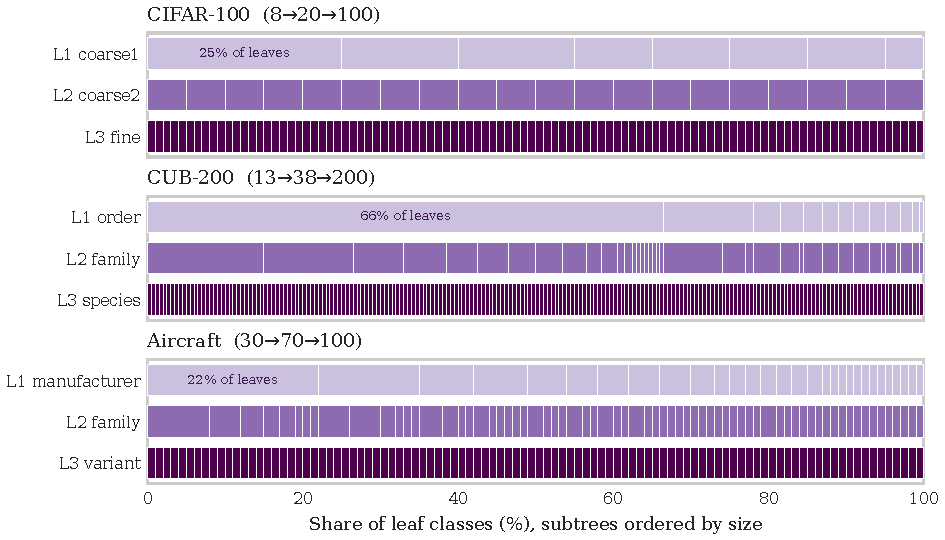
\includegraphics[width=\linewidth]{images/dataset/taxonomy_icicle.pdf}
\caption{Structure of the three taxonomies. Bands are hierarchy levels and
rectangle widths are the shares of leaf classes in each subtree; the horizontal
order ranks subtrees by size.}
\label{fig:taxonomy_icicle}
\end{figure}

In CIFAR-100 every superclass has
five fine classes, but the eight added coarse classes contain between 5 and 25
fine classes. In CUB-200-2011, one top-level class contains 133 of the 200 species
(66.5\%), and the two largest orders contain 78\%. FGVC-Aircraft is the most even
at the top: its largest manufacturer contains 22 of 100 variants. At the lower
transition, however, many families contain only one variant, as shown by the
equal-width family and variant rectangles.

\cref{tab:branching} gives values for both transitions. The last column is
especially useful: a parent with one child requires no choice because its label
already determines the child. On FGVC-Aircraft, 54 of the 70
families (77\%) contain exactly one variant, and 8 of the 13 CUB orders (62\%) contain a single
family. CIFAR-100 has almost none, by construction.

\begin{table}[ht]
\centering
\caption{Branching statistics of the two transitions of each taxonomy. Levels
are numbered from the coarsest ($L_1$) to the finest ($L_3$). ``Single-child
parents'' counts the parents with exactly one child, for which the level pair
carries no decision.}
\label{tab:branching}
\experimenttablesetup
\begin{tabularx}{\linewidth}{@{}L{2.7cm}CCCCCC@{}}
\toprule
\textbf{Dataset} & \textbf{Levels} & \textbf{Parents} & \textbf{Children} & \textbf{Median} & \textbf{Max} & \textbf{Single-child parents} \\
\midrule
CIFAR-100     & $L_1 \to L_2$ & 8  & 20  & 2.0 & 5  & 1 (12\%) \\
CIFAR-100     & $L_2 \to L_3$ & 20 & 100 & 5.0 & 5  & 0 (0\%) \\
\midrule
CUB-200-2011  & $L_1 \to L_2$ & 13 & 38  & 1.0 & 21 & 8 (62\%) \\
CUB-200-2011  & $L_2 \to L_3$ & 38 & 200 & 3.5 & 30 & 12 (32\%) \\
\midrule
FGVC-Aircraft & $L_1 \to L_2$ & 30 & 70  & 2.0 & 8  & 14 (47\%) \\
FGVC-Aircraft & $L_2 \to L_3$ & 70 & 100 & 1.0 & 8  & 54 (77\%) \\
\bottomrule
\end{tabularx}
\end{table}

\subsubsection{Coarse-level information}

Each transition can also be described by the uncertainty about the child after
the parent is known. This is measured in bits by the conditional entropy
$H(\text{child}\mid\text{parent})$. Comparing it with $H(\text{child})$, which
does not use the hierarchy, shows how much information a correct parent provides.
\cref{fig:conditional_entropy} reports both values.

\begin{figure}[ht]
\centering
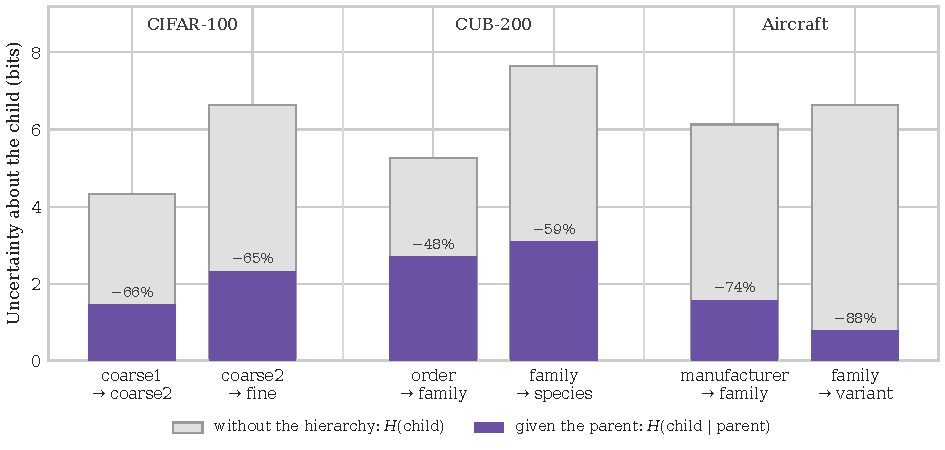
\includegraphics[width=\linewidth]{images/dataset/hierarchy_conditional_entropy.pdf}
\caption{Structural child-class uncertainty at each transition. Coloured bars
show $H(\text{child}\mid\text{parent})$; grey segments show the reduction from
$H(\text{child})$, under a uniform distribution over classes.}
\label{fig:conditional_entropy}
\end{figure}

The datasets differ clearly. On FGVC-Aircraft, choosing one of 100 variants
requires $\log_2 100 = 6.64$ bits without the hierarchy. Once the family is
known, only $0.78$ bits remain, equal to fewer than two likely variants. This
88\% reduction follows from the 54 families with one variant. On CUB-200-2011,
the family-to-species transition leaves $3.10$ of $7.64$ bits, or about nine
likely species, for a 59\% reduction. The order-to-family transition has the
smallest reduction of all six, at 48\%, because one order is much larger than the
others. CIFAR-100 lies between them and has similar reductions at its two
transitions, at 66\% and 65\%.

These values describe the tree alone and assume a uniform distribution over
classes. Weighting by training-image counts
changes every transition by at most $0.13$ bits and leaves CIFAR-100 unchanged,
so sample imbalance has little effect on the reported values. The statistic
measures how much a correct parent constrains its child, not whether a model
learns or benefits from that constraint. On this measure, the parent gives very
strong information for Aircraft, CUB has one dominant branch, and CIFAR-100 has
two more balanced transitions.

\subsubsection{Image resolution and model presets}

\cref{fig:image_geometry} shows the native resolution of the training images. The three
datasets occupy three separate regions: CIFAR-100 collapses into a single point at $32\times32$,
CUB-200-2011 has a median of $500\times375$ pixels, with no sampled image exceeding 500 pixels on
its long side, and FGVC-Aircraft has a median of $1024\times699$ pixels, roughly four times the area
of a CUB image and seven hundred times that of a CIFAR-100 image.

\begin{figure}[ht]
\centering
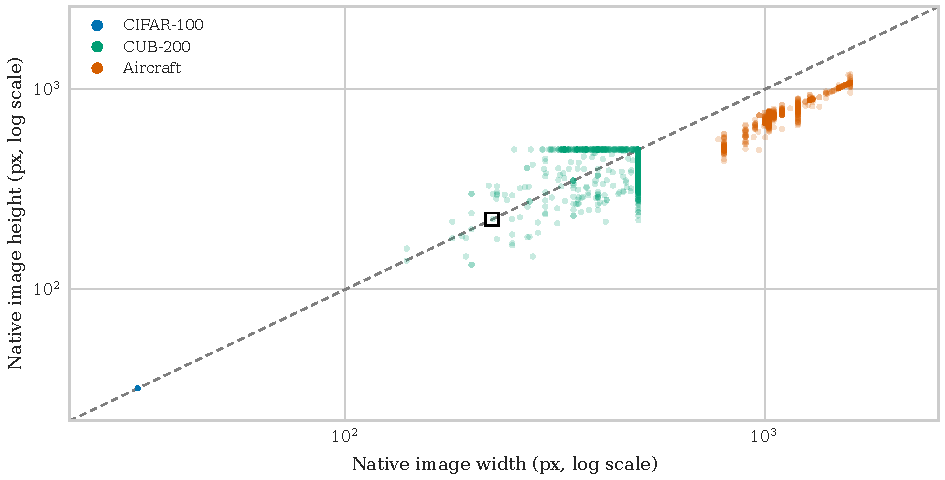
\includegraphics[width=\linewidth]{images/dataset/native_image_geometry.pdf}
\caption{Native resolution of the sampled training images on logarithmic axes.
The diagonal marks square images; the open marker indicates the
$224\times224$ input used by most presets.}
\label{fig:image_geometry}
\end{figure}

The model presets use different input resolutions. CIFAR-100 is
used natively at $32\times32$ by every model, but CUB-200-2011 and FGVC-Aircraft are resized to
$224\times224$ by the H-CAST, Hier-COS and LH-DNN presets, to $448\times448$ by HRN, and to
$64\times64$ by HT-CapsNet. An Aircraft image is thus reduced in area by a factor of roughly 14 for
a $224$-pixel model, 3.6 for HRN, and 175 for HT-CapsNet. A single resolution would make this factor easier to control, but it
would also change the setting for which each baseline was designed. The results
therefore retain the published resolutions and report this limitation.

\subsubsection{Summary}

Four properties of the experimental setting are relevant to the results.

\begin{itemize}[itemsep=2pt, topsep=3pt]
  \item \textbf{Supervision differs by an order of magnitude per class.} CIFAR-100 provides 450
      training images per leaf class against 25--26 for CUB and 33--34 for Aircraft, so the two
      fine-grained
      benchmarks are low-data regimes and CIFAR-100 is not.
  \item \textbf{The trees are unbalanced in different ways.} CUB is dominated by one order covering
      66.5\% of the species. In Aircraft, 77\% of families contain only one
      variant. CIFAR-100 is regular below and deliberately uneven above.
  \item \textbf{The hierarchy provides different amounts of information.} A correct parent
      removes 88\% of the leaf uncertainty on Aircraft, 59\% on CUB, and 65\% on CIFAR-100. The
      datasets therefore test the methods under different conditions.
  \item \textbf{Two experimental factors are not controlled.} Split composition is inherited
      (Aircraft validates on a third of its data, CIFAR-100 on 8\%), and input resolution is
      inherited from each method's published configuration (64, 224, or 448 pixels on the
      fine-grained datasets).
\end{itemize}

The statistics depend on the taxonomies in \cref{sec:hierarchy_construction}.

% ======================================================
%                       METRICS
% ======================================================
\section{Metrics}
\label{ssec:inference_metrics}

\Cref{subsec:metrics} defines and compares the available measures. The
experiments use the five in \cref{tab:metrics_summary}. They measure per-level
accuracy, full-path accuracy, error size and path validity, and they can be
computed from every baseline's decoded output.

\begin{table}[ht]
\centering
\caption{Measures retained for the experiments, with the question each one
answers and the direction of improvement.}
\label{tab:metrics_summary}
\experimenttablesetup
\begin{tabularx}{\linewidth}{@{}L{2.3cm}Y L{1.8cm}@{}}
\toprule
\textbf{Measure} & \textbf{Question answered} & \textbf{Direction} \\
\midrule
$\operatorname{Acc}_l$ & Is level $l$ correct on its own? & Higher \\
wAP & What is the class-count-weighted summary of level accuracies? & Higher \\
FPA & Is the complete predicted path correct? & Higher \\
AHD & How far below the last correct ancestor does the error occur? & Lower \\
TICE & Does the predicted tuple violate a parent--child edge? & Lower \\
\bottomrule
\end{tabularx}
\end{table}

For completeness, let $N$ be the number of examples, $L$ the number of levels,
$C_l$ the number of classes at level $l$, $y_{il}$ and $\hat y_{il}$ the true
and predicted labels, and $\pi_l$ the map from a class at level $l+1$ to its
parent at level $l$. The measures used in the experiments are

\begin{align*}
\operatorname{Acc}_l
&=\frac{1}{N}\sum_{i=1}^{N}\mathbf{1}[\hat y_{il}=y_{il}], \\
\mathrm{wAP}
&=\frac{\sum_{l=1}^{L}C_l\operatorname{Acc}_l}{\sum_{l=1}^{L}C_l}, \\
\mathrm{FPA}
&=\frac{1}{N}\sum_{i=1}^{N}
  \mathbf{1}[\hat y_{il}=y_{il}\ \text{for every }l], \\
\mathrm{AHD}
&=\frac{1}{N}\sum_{i=1}^{N}(L-m_i),
\quad
m_i=\max\bigl\{m\in\{0,\dots,L\}:\hat y_{il}=y_{il}
\ \text{for every }l\leq m\bigr\}, \\
\mathrm{TICE}
&=\frac{1}{N}\sum_{i=1}^{N}
  \mathbf{1}[\exists l<L:\pi_l(\hat y_{i,l+1})\neq\hat y_{il}].
\end{align*}

These formulas recap
\cref{eq:metric_accuracy,eq:metric_wap,eq:metric_fpa,eq:metric_ahd,eq:metric_tice}
so that the experimental tables can be read without returning to the literature
review. FPA is the main measure for checkpoint selection. In wAP, the class counts
$C_l$ are unrelated to the objective weights $w_l$ of
\cref{ssec:problem_objective}; wAP is reported only as a short summary and
never in place of the per-level accuracies. The alternatives are not repeated
here. In this fixed-depth, single-path setting, hP, hR and hF give no extra
information on valid paths. The broader cases handled by HCM do not occur here.
MS is defined only for errors, while HOPS needs a full ranking of the leaves and
mixes accuracy with error size. This study reports those two effects separately.

All five measures are evaluated relative to a chosen cell of the inference grid
of \cref{ssec:inference_grid}. Unless a table states otherwise, results use each
family's native readout and report independent and top-down decoding separately.
For AHD, $m_i$ is explicitly the length of the longest correct prefix, with
$m_i=0$ when the coarsest prediction is wrong. This agrees with the LCA-height
definition for valid paths and extends it to the invalid tuples that independent
decoding can produce.

By \cref{prop:topdown_consistency}, $\mathrm{TICE}$ is identically zero under
top-down decoding, so the useful quantity is
$\mathrm{TICE}_{\text{independent}}$, which measures whether a model produces
an independently decoded valid path without help from the decoder. A comparison of TICE across methods is therefore
meaningful only in the independent column; the top-down column is reported as a
check that the decoder behaves as specified.


% ======================================================================
%                            R E S U L T S
% ======================================================================
%
% RESULT DRAFT. Remaining \tbd cells must be replaced with values produced by
% the evaluation pipeline; no number in this part of the chapter is to be
% transcribed from a plot.
%
% Filling conventions, following \cref{ssec:design_protocol}:
%   * A top-down row is read from the top-down-selected checkpoint and an
%     independent row from the independent-selected checkpoint
%     (\cref{ssec:design_checkpoints}). The two rows of a family may
%     therefore come from different epochs of the same run.
%   * A result is quoted under the family's native cell of the inference grid:
%     node_score for H-CAST, HRN, HT-CapsNet and LH-DNN, subspace_norm for
%     Hier-COS. Rows from any other cell are labelled explicitly.
%   * Every aggregate carries its seed count n; where n > 1 report
%     mean +- sample standard deviation, and compute per-seed differences
%     before averaging whenever the seeds are matched.
%   * Percentages to two decimals, AHD to three, differences in percentage
%     points.
%   * A cell that cannot exist by \cref{ssec:design_support} is marked n/a
%     and is NOT a missing run; a cell that could exist but has not been run
%     is marked \tbd and must be identified locally as an uncompleted run.
%
% Paragraphs marked "% [ANALYSIS]" are deliberately left unwritten: they are
% the places where the numbers are interpreted, and they cannot be drafted
% before the numbers exist.
% ======================================================================

\providecommand{\tbd}{\textcolor{gray}{--}}
\providecommand{\na}{\textit{n/a}}

\section{Baseline comparability}
\label{sec:fidelity}

The five baselines come from separate codebases, frameworks and evaluation
protocols. The unified implementation gives them common data splits, metrics and
checkpoint-selection rules. This section records the source of each baseline,
the shared rules and any differences from the published settings.

Here, \emph{paper-aligned} means that the architecture, objective and inference
rule match the cited source under the checks in
\cref{ssec:fidelity_verification}. It does not mean that the published numbers
are reproduced exactly. The framework, protocol, hardware and seeds may differ.

\subsection{Reference implementations}
\label{ssec:fidelity_anchors}

\begin{table}[htbp]
\centering
\caption{Sources used to audit the local implementations. The revisions fix the
meaning of ``reference implementation'' throughout this chapter.}
\label{tab:fidelity_anchors}
\experimenttablesetup
\begin{tabularx}{\linewidth}{@{}L{2.4cm}YL{2.1cm}L{2.8cm}@{}}
\toprule
\textbf{Family} & \textbf{Reference implementation} & \textbf{Revision} & \textbf{Source framework} \\
\midrule
H-CAST     & \href{https://github.com/pseulki/HCAST}{\texttt{pseulki/HCAST}} & \texttt{b1a222bb} & PyTorch \\
HT-CapsNet & \href{https://github.com/tasrif-khondaker/HT-CapsNet}{\texttt{tasrif-khondaker/HT-CapsNet}} & \texttt{8a0ea23f} & TensorFlow / Keras \\
HRN        & \href{https://github.com/MonsterZhZh/HRN}{\texttt{MonsterZhZh/HRN}} & \texttt{59944e48} & PyTorch \\
Hier-COS   & \href{https://github.com/Depanshu-Sani/Hier-COS}{\texttt{Depanshu-Sani/Hier-COS}} & \texttt{122b01df} & PyTorch \\
LH-DNN     & paper only \cite{fiaschi2024informed} & --- & not released \\
\bottomrule
\end{tabularx}
\end{table}

LH-DNN is the only family without official code. Its local version was built
from the equations, figures and experiment description in
\cite{fiaschi2024informed}. Differences from the paper may therefore come from
this reconstruction.

\subsection{Common evaluation protocol}
\label{ssec:fidelity_protocol}

All families use the same coarse-to-fine label order, dataset splits
and label indices. Validation and test include every sample, and checkpoints are
selected on validation data only. A run retains the mode-specific candidates
defined in \cref{ssec:design_checkpoints}, but every paired post-hoc inference
comparison uses one fixed, independently selected checkpoint. Metrics, logging,
mixed-precision checks and resume validation are also shared.

Every configuration is trained three times with seeds $0$, $1$ and $2$. The
seed changes network initialisation and other random parts of training, but not
the data splits. The CIFAR-100 and CUB-200-2011 validation splits
(\cref{sec:dataset_analysis}) are built once with seed $0$ and reused in every
run. All arms and seeds therefore use the same data. The same three training
seeds are also used for every arm. This is called \emph{matched seeds} in the
rest of the chapter. When two arms share seeds, their difference is computed for
each seed before the results are averaged. Three runs allow a sample standard
deviation to be reported, but they are not enough for a significance test. No
such test is applied
(\cref{ssec:design_threats}).

These choices correct two behaviours present in some reference codebases:
dropping incomplete evaluation batches and selecting results on test data. They
also mean that the experiments below are controlled comparisons inside this
framework, not exact reproductions of the published runs.

\subsection{Model adaptations}
\label{ssec:fidelity_classes}
\label{ssec:fidelity_families}

Three types of difference matter when reading the results. A
\emph{protocol adaptation} applies the common rules above without changing the
main computation of the method. A \emph{local extension}, such as HCC or
lexicographic mode, adds a contribution of this thesis to a baseline. An
\emph{unsupported extrapolation} runs a family on a dataset or hierarchy not
used in its source. Such rows describe the local implementation, not the
published method.

\paragraph{H-CAST.} The CAST and H-CAST components, segmentation path and losses
are kept. The wrapper only converts outputs to the common coarse-to-fine
order. For FGVC-Aircraft, the local hierarchy is built from the official
manufacturer, family and variant annotations because the upstream helper relies
on a repository-local, partly hard-coded taxonomy. Compatibility guards for
current PyTorch and \texttt{timm} versions are covered by tests. HCC and
lexicographic mode are local extensions.

\paragraph{LH-DNN.} The reconstruction follows the reported
$8\to20\to100$ CIFAR hierarchy, large convolutional architecture, detached branch
projections, advantage connections, unweighted level losses and 15-epoch
schedule. CUB-200-2011 and FGVC-Aircraft are extrapolations. On their larger
$224$-pixel inputs, fixed average pooling preserves the paper's input size for
the dense head and prevents that head from growing with image area.

\paragraph{HT-CapsNet.} The TensorFlow/Keras source was ported to PyTorch while
retaining its capsule stages, routing, taxonomy mask, attention, margin loss and
dynamic level weighting. Except for the capsule readout described below, where
the paper and code differ the port follows the released training code. In
particular, it uses
$1-\mathrm{acc}_l^{(t)}\omega_l^{\mathrm{init}}$ inside the dynamic-weight
callback. The paper instead gives
$(1-\mathrm{acc}_l^{(t)})\omega_l^{\mathrm{init}}$; the two versions are derived
and contrasted in \cref{subsec:htcapsnet}. It also retains the saved
taxonomy-temperature settings. The attention implementation is tested against
the Keras projection behaviour.

The post-attention capsule readout is changed to correct a problem in the
published setup. The
paper and released implementation apply layer normalisation to the sum of the
routed capsule and its attention residual. This is incompatible with the
subsequent readout: class evidence is the Euclidean length of each capsule, and
the margin loss compares that length with $m^+=0.9$ and $m^-=0.1$. At the
default layer-normalisation parameters, a $d$-dimensional capsule has
$\lVert\operatorname{LN}(x)\rVert_2\simeq\sqrt{d}$ independently of its input
scale. For the released capsule dimensions $64$, $32$ and $16$, the initial
lengths are therefore approximately $8$, $5.66$ and $4$: they exceed both
margins and are almost constant across classes. The normalisation therefore
removes the length information that the capsule loss uses as evidence that a
class is present.

All HT-CapsNet experiments in this work instead apply the standard capsule
squash function to the same residual sum,
\[
\operatorname{squash}(x)
=\frac{\lVert x\rVert_2^2}{1+\lVert x\rVert_2^2}
  \frac{x}{\lVert x\rVert_2},
\qquad
0\leq\lVert\operatorname{squash}(x)\rVert_2<1.
\]
This change keeps the attention and routing computations and restores the
bounded capsule lengths expected by the margin loss. In a small test that trains
on the same 16 CIFAR-100 images for 60 updates, the
released LayerNorm readout ended with total loss $362.15$ and accuracies
$1.00/0.06/0.00$, whereas changing only this readout to squash ended with loss
$0.082$ and accuracies $1.00/1.00/1.00$ in coarse-to-fine order. This test shows
that the readout causes the failure in this setting, but it is not used as
benchmark evidence.

A separate CIFAR-100 run of the authors' released TensorFlow/Keras code did not
reach the published values during the observed part of training
(\cref{fig:htcapsnet_reproduction}). At
epoch 34 of the planned 200, its coarse-to-fine accuracies were
$26.42/8.60/2.30\%$, still close to the $25/5/1\%$ constant-output floors and
far from the paper's $87.17/80.22/67.58\%$
\cite{noor2025taxonomy}. The run was stopped at that point
and therefore never produced a final test evaluation. This partial run records
the failed reproduction attempt, but it cannot show what would have happened
later in training. The evidence for the LayerNorm problem instead comes from the
calculation above and the small test in which only the readout was changed.

\begin{figure}[htbp]
\centering
\includegraphics[width=\linewidth,trim=0 55bp 0 0,clip]{images/experiments/htcapsnet_upstream_reproduction.png}
\caption{HT-CapsNet readout correction on
CIFAR-100. Blue is the authors' released Keras implementation with LayerNorm,
observed for 34 of 200 epochs; its ``validation'' split is the test set. Orange
is seed 0 of the local squash-corrected port, trained for 100 epochs with a
held-out 10\% validation split. Dotted lines mark the constant-output accuracy
floors and dashed lines the paper's test accuracies. The curves are not a
controlled readout ablation because their frameworks and protocols differ. The
small matched test in the text changes only the readout.}
\label{fig:htcapsnet_reproduction}
\end{figure}

With squash, the three-seed local baseline reaches test accuracies of
$84.52/75.61/61.62\%$ (\cref{tab:results_baseline_cifar}), respectively
$2.65$, $4.61$ and $5.96$ percentage points below the paper. The corrected model
is close to, but does not exactly reproduce, the published result. The
validation protocol may explain part of the remaining gap. The
released code trains on all 50,000 CIFAR-100 training images and reuses the test
set for validation, whereas this work trains on 45,000 and reserves 5,000 for
checkpoint selection. The split alone cannot explain the gap. The local run also
uses 100 epochs and batch size 64, while the released setup uses 200 epochs and
batch size 32. The local code is also a PyTorch port of the released TensorFlow
implementation.

Because squash changes a computation used in both the paper and its source code,
the HT-CapsNet rows report a corrected local version, not an exact reproduction.
The unified CUB hierarchy also
differs from the paper's hierarchy, and FGVC-Aircraft is an extrapolation.

\paragraph{HRN.} The local model retains the ResNet-50 trunk, residual branches,
tree scores, leaf classifier, residual fusion and native sigmoid/softmax readout.
Fine-grained preprocessing and optimisation follow the source. The common
protocol changes evaluation and checkpoint selection; partial-label training is
out of scope, and mixup and cutmix are disabled. CIFAR-100 is an extrapolation
and uses its native $32$-pixel inputs. The HRN baseline throughout the results is
the \texttt{level\_conditional} run. This mode exposes the three differentiable
level objectives required by the mechanism experiments through the chain rule of
\cref{ssec:lex_family_adaptation}; because the terms telescope to the native
objective, the baseline reports the family's own objective rather than a
substitute for it.

\paragraph{Hier-COS.} The taxonomy-node coordinates, fixed orthonormal frame,
backbones, preprocessing and subspace-norm inference are kept. The Hier-COS
baseline throughout the results is the matched global-softmax cross-entropy
reference with regularisation and \texttt{kl\_leaf} weights, rather than the
paper's node-wide KL objective. The released scripts use inconsistent
feature-space flags across datasets, so the local fine-grained preset is a
documented adaptation. The decomposed objectives of
\cref{ssec:lhproj_hiercos} are further local extensions whose cost is measured
separately in \cref{ssec:design_substrate}; the three-level CIFAR hierarchy also
departs from the source's five-level setting.

The unsupported family--dataset settings are therefore HRN on CIFAR-100;
Hier-COS on CUB-200-2011 and on the three-level CIFAR hierarchy; HT-CapsNet on
FGVC-Aircraft and on the unified CUB hierarchy; and LH-DNN on CUB-200-2011 and
FGVC-Aircraft.

\subsection{Verification and limitations}
\label{ssec:fidelity_verification}

Automated tests cover the ported capsule equations and attention shapes, the
taxonomy mask, the HRN objective and schedule, and the model presets. They also
verify that disabling HCC leaves the unconstrained computation unchanged, that
HCC satisfies its hierarchy constraints, that top-down decoding matches a
reference implementation, and that the subspace-norm readout reproduces native
Hier-COS inference.

These tests check the equations, tensor shapes and required properties. They do
not show that a trained local model is numerically identical to a published
checkpoint. The comparisons below do not require such an exact match.

% ======================================================================
\section{Experimental protocol}
\label{sec:results_design}

\subsection{Research questions}
\label{ssec:design_questions}

\paragraph{General question.} Does a coarse-to-fine priority improve
hierarchical classification, and which measures does it improve? If there is a
gain, does it come from the priority itself, or from level weights, model changes
or inference rules? The experiments also test whether applying the constraint at
different points changes the balance between accuracy and consistency.

\cref{tab:design_overview} divides this general question into four research
questions. The last column states what evidence is needed to answer each one. It
does not set the order in which results are presented.

\begin{table}[htbp]
\centering
\caption{Research questions and the evidence required to identify them.}
\label{tab:design_overview}
\experimenttablesetup
\begin{tabularx}{\linewidth}{@{}L{0.8cm}Y Y@{}}
\toprule
& \textbf{Research question} & \textbf{Identifying evidence} \\
\midrule
\textbf{Q1} & Compared with scalar training using the same level weights, does
coarse-to-fine priority improve accuracy, full-path correctness, or structural
consistency?
& Within-family, within-dataset comparison of each applicable priority arm with
its matched \emph{none} baseline, supported by mechanism-activation diagnostics \\
\textbf{Q2} & Is the ordering itself responsible for the effect, or can it be
reproduced by inverted priority or by coarse-heavy scalar weighting? & Matched
\texttt{coarse\_first}, \texttt{fine\_first}, ordinary baseline, and
    coarse-heavy scalar-weighted arms \\
\textbf{Q3} & Do HCC, the LH-projection, and explicit lexicographic mode have
different effects? Do the differences depend on where they act, and do they
arise during training or inference? & Within-family
deltas at the shared mechanism axis, the baseline and gradient-priority
frozen-checkpoint inference grids, trained-HCC versus post-hoc-HCC comparisons,
and separate accounting for the Hier-COS frame, normaliser and weighting
ablations \\
\textbf{Q4} & Under which model families, taxonomies, gradient scales and model
settings does an effect persist? & Repetition across supported family--dataset pairs and the frame, softmax,
    gradient-scale, width, and parameter-form ablations \\
\bottomrule
\end{tabularx}
\end{table}

The three \emph{priority mechanisms} are not mathematically the same. Explicit
lexicographic mode and the LH-projection order gradient contributions, but they
do so at different points. HCC instead applies a one-way constraint to the
outputs. It has a lexicographic form but does not solve the level objectives one
after another. Direct subspace supervision changes the objective without
ordering it, so it is not one of the three mechanisms in Q3. It tests whether a
different training target can change the same metrics without a priority order.

Q1 asks whether there is an effect, and Q2 asks what causes it. Q3 tests whether
the point of application matters and separates training effects from inference
effects. Q4 tests how broadly the result holds. A positive answer to Q1 requires
evidence that the mechanism was active, and Q2--Q4 limit how that answer can be
interpreted.

All claims about cause use comparisons within the same family, dataset,
training recipe and, where available, matched seeds. Cross-family results answer
questions about how well the implementations match their sources and help answer Q4, but they do not
isolate a mechanism because the complete architectures and training recipes
differ. \Cref{sec:fidelity} treats reproducibility and comparability as setup
requirements, not as separate research questions.

\subsection{Checkpoint selection}
\label{ssec:design_checkpoints}

Independent and top-down decoding may favour different training epochs. Every
run therefore retains one checkpoint per decoding mode, selected on the
validation split using the metrics computed under that mode. Candidate
checkpoints are ranked by lexicographic maximisation of
\[
\Big(\;\mathrm{FPA}_{\text{mode}},\;\; -\mathrm{TICE}_{\text{mode}},\;\;
\mathrm{wAP}_{\text{mode}}\;\Big).
\]
Full-path accuracy is compared first. Ties are resolved by lower TICE
and then by higher weighted AP. When hierarchical metrics are unavailable,
deepest-level accuracy is used on its own. Test data are never used for
checkpoint selection.

The protocol separates two types of comparison. End-to-end results use the
checkpoint selected for each decoding mode. They may therefore differ in both
the decoder and the model parameters. Within one decoding mode, alternative
readouts and post-hoc transforms are applied to the same checkpoint: the
independent cells use the independently selected checkpoint and the top-down
cells use the top-down-selected checkpoint. Those comparisons isolate the
readout or transform. Comparisons between the two decoders retain their
selection-specific checkpoints and therefore compare the complete
checkpoint-selection and decoding pipelines; they are not interpreted as a
decoder-only intervention.

\subsection{Identifying mechanism effects}
\label{ssec:design_locus}

The experiments compare four changes with an unmodified baseline: HCC,
explicit lexicographic gradient ordering, the LH-projection, and direct
supervision of taxonomy-subspace scores. They are tested as separate
\emph{experimental conditions} (\cref{sec:methodology_axis}). The study tests
one at a time, not combinations. Each trained change is compared
with its corresponding unmodified family at matched dataset and training recipe.

\paragraph{HCC: training effect or inference correction?} HCC changes the
forward computation both during training and at inference
(\cref{ssec:inference_interaction}). Applying it post hoc to an unconstrained
checkpoint measures its direct effect at inference. Comparing that result with a model
trained under HCC measures the extra effect of using the constraint during
training.

\paragraph{Explicit lexicographic ordering.} The proposed
\texttt{coarse\_first} mode is compared with the baseline and with
\texttt{fine\_first}, which reverses priority while using the same projection
operator (\cref{ssec:lex_modes}). Taxonomy-based level scales are varied
separately. Projection changes gradient directions but does not set the relative
size of the remaining contributions (\cref{ssec:problem_lr}).

\paragraph{LH-projection against explicit ordering.} Both methods implement
coarse-to-fine protection, but at different points of the computation. The
LH-projection acts inside the graph at a branch point; explicit lexicographic
mode combines complete level gradients after backpropagation. They are compared
on Hier-COS with matched frame, loss, weights and seeds. Representation width
and the advantage parameter form are then varied to test which settings the
in-graph method needs (\cref{ssec:lhproj_setting}).

\paragraph{Comparison across points of application.} HCC constrains outputs, the
two lexicographic methods constrain gradients, and direct subspace supervision
changes the objective. Each is compared with the shared \emph{none} condition.
These are separate alternatives. Their combinations are outside the design in
\cref{ssec:design_axis}.

\subsection{Direct supervision of subspace scores}
\label{ssec:design_objective}

This experiment uses Hier-COS only. Other families could use the same target
geometry if they exposed taxonomy-subspace scores, but the implemented loss is
written for Hier-COS outputs and weights. Hier-COS is also the only baseline
whose native decoder already ranks these scores. Its native loss supervises
taxonomy-node coordinates, while inference ranks taxonomy-subspace norms
(\cref{ssec:problem_scores}). Direct subspace supervision changes the training
target but keeps the readout and decoder fixed. In a classifier-head family, the
same objective would also replace the native node-score readout and would test a
different change. That case is not included here.

The minimum target margin decreases from coarse to fine
(\cref{prop:subspace_margin}), so results may depend on the temperature $\tau$.
Only $\tau=0.1$ was evaluated; the planned sweep was not run. The effect of this
missing comparison is discussed in \cref{ssec:results_subspace_tau}. This arm uses
hard path labels, with label smoothing, mixup and cutmix disabled as required by
\cref{ssec:subspace_setting}.

\subsection{Hier-COS adaptations}
\label{ssec:design_substrate}

The LH-projection cannot be added directly to published Hier-COS. It requires
independent level heads, an orthonormal frame that does not mix levels, and a
loss whose level terms depend only on their corresponding heads
(\cref{ssec:lhproj_hiercos}). Two ablations measure the cost of these required
changes. A third then fixes the relative level scale
before the LH-projection is compared with explicit lexicographic training.

\begin{enumerate}
    \item \textbf{Frame.} Dense, block-diagonal and identity frames are compared
    with the readout and node layout fixed. This separates mixing between levels
    from rotation within each level and measures the cost of replacing the
    dense frame before the LH-projection is enabled.
    \item \textbf{Softmax scope.} Global and per-level normalisation are compared
    at the same frame and weights. Explicit lexicographic training only requires
    separate differentiable losses and can retain the global normaliser. The
    LH-projection requires per-level normalisation, because each loss must depend
    on its own branch alone.
    \item \textbf{Level weighting.} Uniform, Hier-COS leaf-heavy and
    class-count-derived weights are evaluated on the LH-projection arm at the
    selected frame and per-level normaliser. The unmodified and
    \texttt{coarse\_first} arms use one fixed rule and are not rerun for every
    weight setting. Only the in-graph method carries the weights into its reserved
    subspace (\cref{ssec:results_lhproj_weight_transfer}). As a result, this test
    cannot fully separate the effect of the weights from their interaction with
    the mechanism. Aircraft also uses the marginal-branching rule, whose largest
    weight is assigned to the middle level.
\end{enumerate}

The frame and softmax ablations first select one LH-compatible configuration per
dataset. The weight ablation is then run on that fixed
configuration in three matched arms: unmodified, \texttt{coarse\_first} and the LH-projection.
This order keeps frame and normaliser changes out of the weight--mechanism
interaction. The frame and softmax steps are reported before
the LH-projection (\cref{sec:results_substrate}); the weight cross is reported
with it (\cref{sec:results_lhprojection}), because the weighting cannot be fixed
on the lexicographic arm and transferred to the in-graph arm.

\subsection{Controls}
\label{ssec:design_controls}

Two controls test other possible explanations for a gain from
coarse-first gradient ordering.

\begin{enumerate}
    \item \textbf{Inverted priority.} \texttt{fine\_first} applies the same
    projection operator as \texttt{coarse\_first}, but reverses the order. It
    separates coarse-first priority from the general effect of
    modifying gradients.
    \item \textbf{Coarse-heavy weighting.} A scalar baseline with greater weight
    on coarse losses tests whether simple reweighting can reproduce any observed
    gain in hierarchical consistency. If it can, projection is not required to
    reach that accuracy--consistency trade-off.
\end{enumerate}

\subsection{Limitations}
\label{ssec:design_threats}

The following limitations affect how the result tables should be read.

\begin{itemize}
    \item \textbf{HT-CapsNet capsule readout.} Every HT-CapsNet arm replaces the
    released post-attention LayerNorm with capsule squash, as explained in
    \cref{ssec:fidelity_classes}. This common correction keeps comparisons
    between local HT-CapsNet arms matched, but it limits direct comparison with
    the published implementation. The local results therefore do not describe
    that implementation without changes.
    \item \textbf{Level weights.} Whenever possible, an intervention and its
    baseline use the same objective weights. H-CAST and HT-CapsNet expose
    unweighted level losses to lexicographic mode, whereas the native HT-CapsNet
    baseline uses dynamic weighting; comparisons that cannot match this variable
    are labelled explicitly.
    \item \textbf{Training budget.} The native HT-CapsNet baseline and its
    explicit lexicographic configuration both use the shared 100-epoch budget,
    not the 200 epochs of the released launcher. The lexicographic arm
    still costs more per epoch because it evaluates and combines three gradients
    per batch; equal epoch counts therefore do not imply equal compute.
    \item \textbf{Backbone and pretraining.} CIFAR experiments use a
    from-scratch wide residual network where supported, whereas fine-grained
    experiments commonly use ImageNet-pretrained backbones. Effects that change
    between these settings are reported as backbone-dependent.
    \item \textbf{Dataset coverage.} The three taxonomies differ substantially,
    and the unsupported family--dataset pairs listed in
    \cref{ssec:fidelity_classes} are not used to make claims about the published
    methods.
    \item \textbf{Cross-family comparison.} Model families also differ in
    backbone, optimiser, augmentation, input resolution and training budget.
    Cross-family tables compare complete implementations. Claims about a
    mechanism use matched comparisons within a family.
    \item \textbf{Hyperparameter search.} One family--dataset setting received an
    automated search over learning rate, weighting and transform choices; the
    others use published or preset values. This asymmetry affects cross-family
    rankings, although no intervention was tuned separately from its baseline.
    \item \textbf{Resource use.} The operation and storage costs of
    explicit lexicographic mode are derived in \cref{ssec:lex_cost}. The matched
    empirical comparison of the baseline, explicit lexicographic mode and the
    LH-projection is structured in \cref{sec:results_computational_cost}; its
    timing protocol and measurements are not yet complete. Until then, the
    chapter does not rank the measured efficiency of the mechanisms.
    \item \textbf{Statistical scope.} Results are descriptive. Means include the
    sample standard deviation and seed count when multiple seeds exist; paired
    differences are computed per seed where possible. No significance test is
    applied. Non-native cells of the inference grid are used only as diagnostics
    and are not selected after the results are seen.
    \item \textbf{Incomplete coverage.} Not every supported configuration was
    run. Missing cells remain marked \tbd in their corresponding tables and are
    treated as unanswered questions, not as negative results.
\end{itemize}

\subsection{Reporting protocol}
\label{ssec:design_protocol}

The following rules are applied throughout the chapter.

\begin{itemize}
    \item \textbf{One mechanism at a time.} The main experiments vary a single
    intervention against a matched baseline.
    \item \textbf{Required changes before mechanisms.} Required changes to
    Hier-COS are evaluated separately before the LH-projection is enabled. Their
    effect is never included in the delta attributed to the projection.
    \item \textbf{Native inference is the main result.} Each family is
    reported under its native readout. Other cells of the inference grid are
    labelled as diagnostics and are not selected after results are known.
    \item \textbf{Both decoders are reported.} Independent and top-down results
    use checkpoints selected for their respective decoding modes
    (\cref{ssec:design_checkpoints}); a decoder is not treated as an intrinsic
    property of a model family.
    \item \textbf{Activation is checked from logs.} HCC is verified through
    \texttt{proj\_constraint\_alpha}. Gradient ordering is verified through the
    logged cosine similarities, removed norms and degeneracy-guard rate. A
    configuration name alone is not evidence that an intervention was active.
    \item \textbf{Metric direction is fixed.} Each metric is read in the
    direction given in \cref{tab:metrics_summary}. Percentage differences
    are expressed in percentage points.
    \item \textbf{Comparisons are descriptive.} Every aggregate reports its seed
    count and, for multiple seeds, the sample standard deviation; paired
    differences are computed seed by seed where possible. No significance test
    is applied. A single-seed result, or a difference smaller than the observed
    seed-to-seed spread, is not used to claim stable superiority. Truncated epoch
    logs are excluded before curves are averaged.
    \item \textbf{A common figure set accompanies every trained mechanism.}
    Each mechanism is accompanied by the independent-decoding validation
    trajectories of FPA, TICE, wAP and AHD, with the mean and one sample
    standard deviation over seeds and the independently selected checkpoint
    marked on every curve; the per-run, per-level training-objective curves
    produced by \texttt{plot\_per\_run\_per\_level\_training\_losses()}; and
    test accuracy by hierarchy level at the independently selected checkpoint,
    produced by \texttt{plot\_final\_level\_test\_accuracy()}. The plotted
    \texttt{loss\_level\_*} values are the configured contributions to that
    run's objective. They support comparisons across depth within one arm, but
    not numerical comparisons between arms whose objectives differ. The main
    section retains the views needed for its argument; redundant endpoint and
    checkpoint-selection views are placed in the supplementary-figures
    appendix.
    \item \textbf{Each constraint mechanism has its own diagnostic.} HCC is
    diagnosed by constraint activation, score displacement, argmax flips and
    ground-truth parent mass; explicit lexicographic training by pre- and
    post-projection gradient cosines, removed norm and guard skips; and the
    LH-projection by its singular spectrum, effective rank and remaining
    unused representation capacity. Direct subspace supervision changes only the
    objective and therefore uses the common metric, loss and level-accuracy
    figures without an additional mechanism-specific diagnostic. FPA--TICE
    trade-off figures are kept for the later comparison and are not part of
    this common per-mechanism set.
\end{itemize}

\subsection{Experiment overview}
\label{sec:results_campaign}

The results are presented in the following order:

\begin{enumerate}
    \item \Cref{sec:results_baselines} reports the unmodified reference for
    each family.
    \item \Cref{sec:results_inference} applies alternative readouts, HCC and both
    decoders to frozen baseline checkpoints only. This measures inference-time
    effects before the trained changes are considered.
    \item \Cref{sec:results_hcc,sec:results_subspace,sec:results_lex} compare
    three directly trained interventions with their matched baselines, ordered by
    where each acts: on the outputs, on the objective, then on the gradient.
    \item \Cref{sec:results_substrate} changes the Hier-COS frame and normaliser
    once. It selects an LH-compatible configuration and measures the cost of the
    change. Everything before it uses the published dense,
    globally normalised configuration.
    \item \Cref{sec:results_lhprojection} reports the LH-projection on that
    configuration. It is compared first with explicit lexicographic mode, then
    with different level weights on each arm, and finally across the CIFAR-100
    backbone-capacity ladder.
    \item \Cref{sec:results_mechanisms} places the four alternative
    interventions in one comparison.
    \item \Cref{sec:results_inference_priority} returns to the inference grid on
    the explicit lexicographic and LH-projection checkpoints, after both
    mechanisms and their matched comparison have been established.
    \item \Cref{sec:results_computational_cost} compares model size and training
    cost for the matched baseline, explicit lexicographic and LH-projection arms.
    \item \Cref{sec:results_summary} summarises the conclusions supported by the
    results and lists the remaining limitations.
\end{enumerate}

The target protocol of \cref{ssec:fidelity_protocol} uses three seeds per table
row. Each table reports the number of completed seeds in the $n$ column when it
varies by row, and in the caption otherwise. Incomplete cells remain marked
until all planned runs are complete.
\cref{tab:framework_support} fixes which configurations a family does not
admit at all. Supported configurations that were not run are listed in the
corresponding result section and are not treated as negative evidence.

% ======================================================================
\section{Unified baselines}
\label{sec:results_baselines}

Before testing the proposed interventions, two reference points are needed: how
accurately each family predicts at each hierarchy level, and how often its
independent predictions already form a consistent path. This section reports
both on the common splits and taxonomies of \cref{sec:datasets}. In these
baselines, HCC, direct subspace supervision, explicit lexicographic ordering and
the LH-projection are all inactive; the exact family-specific configurations are
documented in \cref{sec:fidelity}.

The later mechanism claims use seed-matched differences within the same family.
Comparisons across families instead locate the complete implementations in the
accuracy--consistency space; they are descriptive because architecture and
training recipe remain family-specific (\cref{ssec:fidelity_families}).

\subsection{Results}
\label{ssec:results_baseline_datasets}

\newcommand{\baselinemeanstd}[2]{\(#1\,{\scriptstyle\pm #2}\)}

All table entries are the mean $\pm$ sample standard deviation over seeds
$0$, $1$ and $2$.
%
% Tables and figures in this section are produced by
% notebooks/model_comparison_all_datasets.ipynb. Its setup cell sets
%   FIGURE_DIR = docs/images/experiments/baseline/
% so re-running the notebook rewrites these PDFs in place; there is no separate
% staging step for this section.
%
% Do NOT run `scripts/stage_thesis_figures.py baseline` to refresh them. That
% group copies from /scratch/.../analysis/model_analysis/comparison/figures/,
% which the notebook no longer writes to, and would overwrite the current
% five-family PDFs with an older four-family export. Use the script for the
% `subspace` group only.
%
% The validation and per-level loss trajectories are supplementary figures in
% capitoli/appendiceA.tex. The main section retains only the endpoint and
% cross-model comparison figures used directly by the analysis below.

\begin{table}[htbp]
\centering
\caption{Baseline test results on CIFAR-100 ($8\to20\to100$).}
\label{tab:results_baseline_cifar}
\resulttablesetup
\begin{tabularx}{\linewidth}{@{}L{2.2cm}|CCC|C|C|C|C@{}}
\toprule
\textbf{Family} & $\mathrm{Acc}_1\uparrow$ & $\mathrm{Acc}_2\uparrow$ & $\mathrm{Acc}_3\uparrow$ & $\mathrm{wAP}\uparrow$ & $\mathrm{FPA}\uparrow$ & $\mathrm{AHD}\downarrow$ & $\mathrm{TICE}\downarrow$ \\
\midrule
H-CAST    & \baselinemeanstd{\underline{90.82}}{0.32} & \baselinemeanstd{\underline{85.20}}{0.39} & \baselinemeanstd{\underline{75.94}}{0.20} & \baselinemeanstd{\underline{78.31}}{0.14} & \baselinemeanstd{\underline{73.48}}{0.19} & \baselinemeanstd{\underline{0.511}}{0.008} & \baselinemeanstd{\underline{7.61}}{0.29} \\
Hier-COS  & \baselinemeanstd{\mathbf{91.35}}{0.06} & \baselinemeanstd{\mathbf{86.87}}{0.21} & \baselinemeanstd{\mathbf{77.80}}{0.21} & \baselinemeanstd{\mathbf{80.07}}{0.20} & \baselinemeanstd{\mathbf{77.52}}{0.16} & \baselinemeanstd{\mathbf{0.444}}{0.003} & \baselinemeanstd{\mathbf{1.04}}{0.04} \\
HRN       & \baselinemeanstd{84.65}{0.12} & \baselinemeanstd{77.16}{0.12} & \baselinemeanstd{70.38}{0.24} & \baselinemeanstd{72.33}{0.19} & \baselinemeanstd{61.76}{0.34} & \baselinemeanstd{0.804}{0.006} & \baselinemeanstd{20.45}{0.17} \\
HT-CapsNet & \baselinemeanstd{84.52}{0.02} & \baselinemeanstd{75.61}{0.10} & \baselinemeanstd{61.62}{0.03} & \baselinemeanstd{65.24}{0.04} & \baselinemeanstd{59.87}{0.21} & \baselinemeanstd{0.809}{0.002} & \baselinemeanstd{7.63}{0.43} \\
LH-DNN    & \baselinemeanstd{74.43}{0.49} & \baselinemeanstd{63.25}{0.65} & \baselinemeanstd{51.40}{0.58} & \baselinemeanstd{54.69}{0.58} & \baselinemeanstd{45.57}{0.48} & \baselinemeanstd{1.199}{0.015} & \baselinemeanstd{17.90}{0.44} \\
\bottomrule
\end{tabularx}
\end{table}

\begin{table}[htbp]
\centering
\caption{Baseline test results on CUB-200-2011 ($13\to38\to200$).}
\label{tab:results_baseline_cub}
\resulttablesetup
\begin{tabularx}{\linewidth}{@{}L{2.2cm}|CCC|C|C|C|C@{}}
\toprule
\textbf{Family} & $\mathrm{Acc}_1\uparrow$ & $\mathrm{Acc}_2\uparrow$ & $\mathrm{Acc}_3\uparrow$ & $\mathrm{wAP}\uparrow$ & $\mathrm{FPA}\uparrow$ & $\mathrm{AHD}\downarrow$ & $\mathrm{TICE}\downarrow$ \\
\midrule
H-CAST    & \baselinemeanstd{\mathbf{98.49}}{0.14} & \baselinemeanstd{\mathbf{94.36}}{0.11} & \baselinemeanstd{\underline{83.09}}{0.16} & \baselinemeanstd{\underline{85.59}}{0.13} & \baselinemeanstd{\mathbf{81.27}}{0.33} & \baselinemeanstd{\mathbf{0.262}}{0.002} & \baselinemeanstd{\underline{5.24}}{0.41} \\
Hier-COS  & \baselinemeanstd{96.85}{0.11} & \baselinemeanstd{90.51}{0.13} & \baselinemeanstd{76.38}{0.41} & \baselinemeanstd{79.58}{0.34} & \baselinemeanstd{76.15}{0.42} & \baselinemeanstd{0.366}{0.006} & \baselinemeanstd{\mathbf{0.60}}{0.19} \\
HRN       & \baselinemeanstd{\underline{98.00}}{0.30} & \baselinemeanstd{\underline{93.91}}{0.22} & \baselinemeanstd{\mathbf{83.49}}{0.10} & \baselinemeanstd{\mathbf{85.82}}{0.10} & \baselinemeanstd{\underline{80.56}}{0.29} & \baselinemeanstd{\underline{0.285}}{0.009} & \baselinemeanstd{6.21}{0.14} \\
HT-CapsNet & \baselinemeanstd{83.67}{0.20} & \baselinemeanstd{56.56}{0.54} & \baselinemeanstd{28.60}{0.93} & \baselinemeanstd{35.68}{0.79} & \baselinemeanstd{24.48}{0.74} & \baselinemeanstd{1.372}{0.010} & \baselinemeanstd{24.43}{1.09} \\
LH-DNN    & \baselinemeanstd{71.30}{0.54} & \baselinemeanstd{30.62}{1.09} & \baselinemeanstd{5.41}{0.55} & \baselinemeanstd{12.64}{0.61} & \baselinemeanstd{2.33}{0.23} & \baselinemeanstd{1.996}{0.015} & \baselinemeanstd{63.05}{1.97} \\
\bottomrule
\end{tabularx}
\end{table}

\begin{table}[htbp]
\centering
\caption{Baseline test results on FGVC-Aircraft ($30\to70\to100$).}
\label{tab:results_baseline_aircraft}
\resulttablesetup
\begin{tabularx}{\linewidth}{@{}L{2.2cm}|CCC|C|C|C|C@{}}
\toprule
\textbf{Family} & $\mathrm{Acc}_1\uparrow$ & $\mathrm{Acc}_2\uparrow$ & $\mathrm{Acc}_3\uparrow$ & $\mathrm{wAP}\uparrow$ & $\mathrm{FPA}\uparrow$ & $\mathrm{AHD}\downarrow$ & $\mathrm{TICE}\downarrow$ \\
\midrule
H-CAST    & \baselinemeanstd{\mathbf{93.31}}{0.12} & \baselinemeanstd{87.57}{0.51} & \baselinemeanstd{72.90}{1.05} & \baselinemeanstd{81.09}{0.61} & \baselinemeanstd{70.73}{1.04} & \baselinemeanstd{0.492}{0.013} & \baselinemeanstd{\underline{9.09}}{0.10} \\
Hier-COS  & \baselinemeanstd{92.22}{0.05} & \baselinemeanstd{\underline{88.10}}{0.33} & \baselinemeanstd{\mathbf{81.55}}{0.52} & \baselinemeanstd{\mathbf{85.44}}{0.37} & \baselinemeanstd{\mathbf{81.40}}{0.52} & \baselinemeanstd{\mathbf{0.384}}{0.008} & \baselinemeanstd{\mathbf{0.78}}{0.13} \\
HRN       & \baselinemeanstd{\underline{92.64}}{0.37} & \baselinemeanstd{\mathbf{88.46}}{0.43} & \baselinemeanstd{\underline{79.37}}{0.24} & \baselinemeanstd{\underline{84.54}}{0.24} & \baselinemeanstd{\underline{75.65}}{0.24} & \baselinemeanstd{\underline{0.460}}{0.009} & \baselinemeanstd{11.21}{0.18} \\
HT-CapsNet & \baselinemeanstd{64.06}{2.49} & \baselinemeanstd{52.63}{2.13} & \baselinemeanstd{42.56}{1.92} & \baselinemeanstd{49.31}{2.07} & \baselinemeanstd{39.03}{2.06} & \baselinemeanstd{1.467}{0.069} & \baselinemeanstd{20.28}{1.21} \\
LH-DNN    & \baselinemeanstd{26.65}{0.49} & \baselinemeanstd{13.42}{0.17} & \baselinemeanstd{7.13}{0.37} & \baselinemeanstd{12.26}{0.20} & \baselinemeanstd{1.96}{0.23} & \baselinemeanstd{2.615}{0.004} & \baselinemeanstd{80.71}{1.31} \\
\bottomrule
\end{tabularx}
\end{table}

\FloatBarrier

\paragraph{CIFAR-100.} Hier-COS leads every reported metric in
\cref{tab:results_baseline_cifar}: its FPA is $77.52\%$ and its TICE is
$1.04\%$. H-CAST is second on both measures, with $73.48\%$ FPA and $7.61\%$
TICE. The separation between the three strongest families is already visible at
the coarsest level and changes little by the finest level, as shown in
\cref{fig:baseline_final_level_accuracy}.

\paragraph{CUB-200-2011.} The lead is divided among three families
(\cref{tab:results_baseline_cub}). H-CAST has the best coarse and middle
accuracies, FPA ($81.27\%$) and AHD; HRN has the best fine accuracy ($83.49\%$)
and wAP. Hier-COS instead has by far the lowest TICE ($0.60\%$), compared with
$5.24\%$ for H-CAST and $6.21\%$ for HRN. Thus the most consistent model is not
the most accurate one on this dataset.

\paragraph{FGVC-Aircraft.} Hier-COS leads fine accuracy, wAP, FPA, AHD and TICE
in \cref{tab:results_baseline_aircraft}, reaching $81.40\%$ FPA with only
$0.78\%$ TICE. HRN is second in FPA at $75.65\%$, while H-CAST reaches
$70.73\%$. H-CAST retains the best coarse accuracy and HRN the best middle-level
accuracy, but \cref{fig:baseline_final_level_accuracy} shows that the ranking
separates most strongly at the finest level.

\FloatBarrier
\begin{figure}[htbp]
\centering
\includegraphics[width=\basefigwidth]{images/experiments/baseline/comparison_final_level_accuracy.pdf}
\caption{Test accuracy at the selected checkpoints, resolved by hierarchy level.}
\label{fig:baseline_final_level_accuracy}
\end{figure}

\paragraph{Overall pattern.} Across datasets, Hier-COS is the strongest baseline
for fine accuracy, wAP, FPA and AHD, leading each on CIFAR-100 and Aircraft; it
is also the TICE leader on all three datasets. H-CAST leads coarse accuracy on
the two fine-grained datasets and provides the best FPA and AHD on CUB. No
family leads middle-level accuracy consistently: Hier-COS, H-CAST and HRN each
lead one dataset. The FPA--TICE view in
\cref{fig:baseline_cross_model_tradeoff} makes the main distinction clear:
Hier-COS dominates on CIFAR-100 and Aircraft, whereas CUB has two complementary
operating points. H-CAST gains $5.12$~pp in FPA over Hier-COS, while Hier-COS
reduces TICE by $4.64$~pp.

\FloatBarrier
\begin{figure}[htbp]
\centering
\includegraphics[width=0.8\linewidth]{images/experiments/baseline/cross_model_fpa_tice_native_independent.pdf}
\caption[Cross-model baseline FPA--TICE trade-off]{Cross-model baseline
FPA--TICE trade-off under independent decoding and each family's native
readout. Large markers are three-seed means, small markers are individual
seeds, and ellipses show one sample standard deviation with the observed
FPA--TICE covariance. Higher FPA and lower TICE are preferable, so improvement
is towards the upper left.}
\label{fig:baseline_cross_model_tradeoff}
\end{figure}

\paragraph{LH-DNN and HT-CapsNet.} LH-DNN falls behind the other families even
on CIFAR-100 ($45.57\%$ FPA) and nearly collapses on CUB and Aircraft, where FPA
is $2.33\%$ and $1.96\%$. Its supplementary validation curves are still rising
when the 15-epoch schedule ends, so these results show that the evaluated recipe
does not transfer to the fine-grained datasets, not that the architecture could
not do so with a different training budget
(\cref{fig:baseline_validation_cub,fig:baseline_validation_aircraft}).
HT-CapsNet is more competitive on CIFAR-100, with $59.87\%$ FPA and $7.63\%$
TICE, but deteriorates on CUB ($24.48\%$ FPA, $24.43\%$ TICE) and Aircraft
($39.03\%$ FPA, $20.28\%$ TICE). The adaptations and unsupported settings that
limit both comparisons are documented in \cref{ssec:fidelity_classes}.

% Keep the two main-text baseline figures inside this section.
\FloatBarrier


% ======================================================================
\section{Baseline inference study}
\label{sec:results_inference}

All results in this section use the frozen baseline checkpoints of
\cref{sec:results_baselines}. No parameters are trained, no loss is constructed,
and all cells of one checkpoint come from a shared forward pass
(\cref{ssec:inference_grid}). Within a decoder, changing the readout or the
post-hoc transform holds the parameter state fixed and isolates that inference
choice. Comparisons between decoders instead use the checkpoint selected for
the corresponding mode, as required by \cref{ssec:design_checkpoints}; they
compare complete selection-and-decoding pipelines. A trained mechanism must
improve beyond the corresponding post-hoc effect before the difference can be
attributed to learning. Checkpoints trained with a mechanism are deliberately
excluded here: the same analysis is resumed only after all mechanism results,
in \cref{sec:results_inference_priority}, for the explicit lexicographic and
LH-projection arms.

The section varies one factor of the inference grid at a time, in the order in
which \cref{sec:methodology_inference} defines them: the readout first, then the
decoder, then the post-hoc transform. \Cref{ssec:results_readout} transplants
the taxonomy-subspace readout onto families that were never trained for it and
\cref{ssec:results_levels} identifies, level by level, the mechanism behind what
it buys. \Cref{ssec:results_decoder} then asks what top-down decoding still
contributes once a readout has been chosen, and \cref{ssec:results_posthoc}
closes the grid with the HCC transform.

\Cref{tab:results_inference_grid} carries the untransformed half of the grid ---
both readouts crossed with both decoders, on all three datasets --- so that the
readout comparison of \cref{ssec:results_readout} and the decoder comparison of
\cref{ssec:results_decoder} can both be read off the same fifteen rows. Only FPA
and TICE are tabulated: they are the two axes of the trade the section is about,
and FPA is the checkpoint selection metric (\cref{ssec:inference_metrics}). wAP
and AHD are omitted as summaries of quantities already shown; the complete
values for every untransformed cell are retained in
\cref{tab:app_results_inference_wap_ahd}. Per-level accuracies enter through
\cref{fig:baseline_readout_level}, where they answer a specific question. TICE
is quoted only under independent decoding, because
\cref{prop:topdown_consistency} makes it identically zero under top-down
decoding.

Every subspace-norm result below is computed in probability space. H-CAST,
LH-DNN and HT-CapsNet coordinates are mapped through a level-wise softmax, HRN
through sigmoid at its two tree levels and softmax at its leaf head, and
Hier-COS coordinates are left unchanged (\cref{ssec:inference_readout}). This
prevents the norm from treating a large negative rejection logit as positive
evidence. All aggregates are means plus one sample standard deviation over the
three seeds.

\begin{table}[htbp]
\centering
\caption{Untransformed inference grid on the frozen baselines: both readouts
crossed with both decoders. Each decoder is read from its own
validation-selected checkpoint; within a decoder the two readouts share one
parameter state, so a left-to-right change is an inference effect. TICE is
identically zero under top-down decoding and is not repeated. Node score is
native for all families except Hier-COS, for which subspace norm is native.
Entries are three-seed mean $\pm$ sample standard deviation.}
\label{tab:results_inference_grid}
\resulttablesetup
\begin{tabularx}{\linewidth}{@{}L{2.0cm}|CCC|CCC@{}}
\toprule
& \multicolumn{3}{c}{\texttt{node\_score}} & \multicolumn{3}{c}{\texttt{subspace\_norm}} \\
\cmidrule(lr){2-4}\cmidrule(l){5-7}
& \multicolumn{2}{c}{independent} & top-down & \multicolumn{2}{c}{independent} & top-down \\
\cmidrule(lr){2-3}\cmidrule(lr){4-4}\cmidrule(lr){5-6}\cmidrule(l){7-7}
\textbf{Family} & FPA$\uparrow$ & TICE$\downarrow$ & FPA$\uparrow$ & FPA$\uparrow$ & TICE$\downarrow$ & FPA$\uparrow$ \\
\midrule
\multicolumn{7}{@{}l}{\textbf{CIFAR-100} ($8\to20\to100$)} \\
H-CAST     & \baselinemeanstd{73.48}{0.19} & \baselinemeanstd{7.61}{0.29} & \baselinemeanstd{75.01}{0.18} & \baselinemeanstd{75.34}{0.05} & \baselinemeanstd{0.21}{0.03} & \baselinemeanstd{75.32}{0.12} \\
Hier-COS   & \baselinemeanstd{77.21}{0.13} & \baselinemeanstd{2.32}{0.05} & \baselinemeanstd{77.74}{0.18} & \baselinemeanstd{77.52}{0.16} & \baselinemeanstd{1.04}{0.04} & \baselinemeanstd{77.74}{0.14} \\
HRN        & \baselinemeanstd{61.76}{0.34} & \baselinemeanstd{20.45}{0.17} & \baselinemeanstd{65.32}{0.76} & \baselinemeanstd{69.19}{0.29} & \baselinemeanstd{0.28}{0.03} & \baselinemeanstd{69.20}{0.55} \\
HT-CapsNet & \baselinemeanstd{59.87}{0.21} & \baselinemeanstd{7.63}{0.43} & \baselinemeanstd{60.76}{0.23} & \baselinemeanstd{60.60}{0.17} & \baselinemeanstd{1.95}{0.06} & \baselinemeanstd{60.73}{0.24} \\
LH-DNN     & \baselinemeanstd{45.57}{0.48} & \baselinemeanstd{17.90}{0.44} & \baselinemeanstd{47.82}{0.51} & \baselinemeanstd{49.83}{0.69} & \baselinemeanstd{0.44}{0.04} & \baselinemeanstd{49.92}{0.66} \\
\midrule
\multicolumn{7}{@{}l}{\textbf{CUB-200-2011} ($13\to38\to200$)} \\
H-CAST     & \baselinemeanstd{81.27}{0.33} & \baselinemeanstd{5.24}{0.41} & \baselinemeanstd{82.68}{0.15} & \baselinemeanstd{83.02}{0.15} & \baselinemeanstd{0.03}{0.02} & \baselinemeanstd{83.02}{0.15} \\
Hier-COS   & \baselinemeanstd{75.79}{0.46} & \baselinemeanstd{2.36}{0.04} & \baselinemeanstd{76.13}{0.52} & \baselinemeanstd{76.15}{0.42} & \baselinemeanstd{0.60}{0.19} & \baselinemeanstd{76.21}{0.47} \\
HRN        & \baselinemeanstd{80.56}{0.29} & \baselinemeanstd{6.21}{0.14} & \baselinemeanstd{81.73}{0.38} & \baselinemeanstd{83.31}{0.24} & \baselinemeanstd{0.10}{0.02} & \baselinemeanstd{83.20}{0.36} \\
HT-CapsNet & \baselinemeanstd{24.48}{0.74} & \baselinemeanstd{24.43}{1.09} & \baselinemeanstd{26.56}{0.79} & \baselinemeanstd{21.14}{1.18} & \baselinemeanstd{25.95}{1.44} & \baselinemeanstd{21.53}{1.02} \\
LH-DNN     & \baselinemeanstd{2.33}{0.23} & \baselinemeanstd{63.05}{1.97} & \baselinemeanstd{3.66}{0.31} & \baselinemeanstd{3.85}{0.57} & \baselinemeanstd{1.05}{0.17} & \baselinemeanstd{4.00}{0.39} \\
\midrule
\multicolumn{7}{@{}l}{\textbf{FGVC-Aircraft} ($30\to70\to100$)} \\
H-CAST     & \baselinemeanstd{70.73}{1.04} & \baselinemeanstd{9.09}{0.10} & \baselinemeanstd{73.47}{0.92} & \baselinemeanstd{73.67}{0.77} & \baselinemeanstd{0.14}{0.06} & \baselinemeanstd{73.60}{0.83} \\
Hier-COS   & \baselinemeanstd{80.86}{0.61} & \baselinemeanstd{2.91}{0.29} & \baselinemeanstd{81.66}{0.46} & \baselinemeanstd{81.40}{0.52} & \baselinemeanstd{0.78}{0.13} & \baselinemeanstd{81.74}{0.43} \\
HRN        & \baselinemeanstd{75.65}{0.24} & \baselinemeanstd{11.21}{0.18} & \baselinemeanstd{78.22}{0.72} & \baselinemeanstd{79.97}{0.41} & \baselinemeanstd{0.19}{0.12} & \baselinemeanstd{79.95}{0.48} \\
HT-CapsNet & \baselinemeanstd{39.03}{2.06} & \baselinemeanstd{20.28}{1.21} & \baselinemeanstd{41.81}{1.98} & \baselinemeanstd{31.85}{2.12} & \baselinemeanstd{41.17}{1.50} & \baselinemeanstd{32.44}{1.76} \\
LH-DNN     & \baselinemeanstd{1.96}{0.23} & \baselinemeanstd{80.71}{1.31} & \baselinemeanstd{3.85}{0.38} & \baselinemeanstd{4.94}{0.11} & \baselinemeanstd{4.71}{0.77} & \baselinemeanstd{5.23}{0.56} \\
\bottomrule
\end{tabularx}
\end{table}

\subsection{Node score vs. subspace norm}
\label{ssec:results_readout}

Hier-COS bundles a frozen orthonormal frame, a subspace-norm readout and a level
regulariser, and the published narrative attaches the benefit to the frame
(\cref{ssec:design_substrate}). Because the readout is definable on any family
(\cref{ssec:inference_readout}), half of that bundle can be tested directly:
the subspace-norm rule is applied here to checkpoints that were never trained
with a frame at all. A gain that survives the transplant belongs to the readout;
one that does not is evidence for the frame, which the ladder of
\cref{ssec:results_frame} then localises further.

\begin{figure}[p]
\centering
\includegraphics[width=\linewidth]{images/experiments/inference/cross_model_fpa_tice_subspace_norm_independent.pdf}
\caption[Cross-model trade-off under subspace-norm inference]{Cross-model
FPA--TICE trade-off when the three leading frozen baselines --- H-CAST, HRN and
Hier-COS --- are read by the probability-space subspace norm and decoded
independently. LH-DNN and HT-CapsNet are omitted from this figure to resolve the
competitive region but remain reported in \cref{tab:results_inference_grid}.
Plotting conventions are those of
\cref{fig:baseline_cross_model_tradeoff}. The same independently selected
checkpoints are used in both figures, so movement between them is a readout
effect within each run; comparisons between families remain comparisons of
complete recipes.}
\label{fig:baseline_cross_model_tradeoff_subspace}
\end{figure}

Read across the independent columns of \cref{tab:results_inference_grid},
the subspace norm raises FPA and lowers TICE in thirteen of the fifteen rows,
and all three seeds agree on the direction of every FPA change. The FPA gains
run from $0.31$~pp for Hier-COS on CIFAR-100, whose native readout this already
is, to $7.43$~pp for HRN on the same dataset; the TICE reductions run to
$20.16$~pp for that HRN row and to $62.01$ and $76.00$~pp for LH-DNN on CUB and
Aircraft.

What the readout does is best stated as a single quantity. Under independent
decoding a model can predict the correct leaf and still fail FPA, because the
ancestors it predicts separately do not lie on that leaf's path; the size of
that failure is $\mathrm{Acc}_3-\mathrm{FPA}$, which top-down decoding
drives to exactly zero by construction. At the node-score readout this gap is
$0.59$--$8.62$~pp across the fifteen rows. At the subspace norm it is
$0.01$--$0.36$~pp in thirteen of them. The readout therefore reaches, without a
decoder, the property that top-down decoding exists to guarantee. LH-DNN on
Aircraft shows the mechanism at its clearest: only $27.6\%$ of its correct
leaves sat on a correct path under node scores, against $95.3\%$ under the
subspace norm, which is why its FPA rises from $1.96$ to $4.94\%$ even though
its fine accuracy falls.

The two rules are alternatives in a precise sense, and the terms are used that
way throughout. Top-down decoding is the \emph{hard} rule: it makes an
inconsistent path unreachable, by restricting each level's argmax to the
children of the level above. The subspace norm is its \emph{soft} counterpart:
it forbids nothing, and instead folds a node's ancestors into its own score, so
that a path whose levels disagree is outranked rather than excluded.
\Cref{ssec:results_decoder} measures what the hard rule still adds once the soft
one is in place.

The two exceptions are both HT-CapsNet fine-grained extrapolations. Its CUB FPA
falls by $3.34$~pp and its Aircraft FPA by $7.18$~pp, while TICE rises by $1.51$
and $20.89$~pp; the leaf-to-path gap moves the wrong way as well, to $5.87$ and
$10.09$~pp. \Cref{fig:baseline_readout_level} locates the cause at the coarsest
level. A coarse subspace contains all descendant coordinates, so its norm
exposes the upper prediction to subtree size and to the calibration of both
lower-level heads. The observation is therefore consistent with a poorly
calibrated identity-frame transplant on the imbalanced fine-grained taxonomies;
it does not establish whether taxonomy shape or HT-CapsNet's $64$-pixel
extrapolation is the primary cause.

\Cref{fig:baseline_cross_model_tradeoff_subspace} shows that the readout also
changes the cross-family Pareto relation. On CIFAR-100, Hier-COS retains the
largest FPA ($77.52\%$), but H-CAST now has lower TICE ($0.21\%$ against
$1.04\%$), so both are Pareto-optimal. On CUB, HRN moves from being dominated by
H-CAST to the largest FPA ($83.31\%$); H-CAST retains the lower TICE ($0.03\%$
against $0.10\%$), and the two dominate Hier-COS. On Aircraft, Hier-COS, HRN and
H-CAST all lie on the frontier: respectively $(81.40,0.78)$, $(79.97,0.19)$ and
$(73.67,0.14)$ in $(\mathrm{FPA},\mathrm{TICE})$ percent. Put against
native readouts, the rule narrows HRN's Aircraft FPA gap to Hier-COS from
$5.75$~pp --- Hier-COS at its native subspace norm against HRN at its native
node score --- to $1.43$~pp once both are read the same way. It does not
produce a single winner on both axes.

These transplants identify a readout effect, not a frame effect. In particular,
the gains for H-CAST, HRN and LH-DNN show that a non-identity orthonormal frame
is not necessary for subspace aggregation to help a frozen checkpoint. They do
not show that Hier-COS's frame is unnecessary during training; that question
requires the controlled frame ladder of \cref{ssec:results_frame}. Nor may the
gain be read as better recognition: the next subsection splits the same paired
change per level, and finds that it is bought at the coarse and middle levels
and often paid for at the leaf.

\subsection{Where the subspace readout acts}
\label{ssec:results_levels}

FPA alone cannot say which of two mechanisms produces the gain of
\cref{ssec:results_readout}. Better leaf recognition and cross-level
reconciliation are both consistent with a higher FPA, and they differ in their
signature across the levels: the first would raise $\mathrm{Acc}_3$, while
the second would raise $\mathrm{Acc}_1$ and $\mathrm{Acc}_2$ and may
spend part of the leaf to do it. \Cref{fig:baseline_readout_level} separates
them by splitting the same paired change per level. Level accuracies are shown
here rather than tabulated because the claim is about the sign pattern across
three levels within a row, which is what the figure makes directly visible.

\begin{figure}[p]
\centering
\includegraphics[width=\linewidth]{images/experiments/inference/baseline_readout_level_gain.pdf}
\caption[Per-level accuracy change from node score to subspace norm]{Per-level
accuracy change when a frozen baseline is re-read with the probability-space
subspace norm instead of its node score, under independent decoding. Each bar is
$\mathrm{Acc}^{\text{sub}}_l-\mathrm{Acc}^{\text{node}}_l$ in
percentage points, formed per seed and then averaged over the three seeds; error
bars are the sample standard deviation of that paired per-seed effect and a
dagger marks an effect whose sign is not shared by all three seeds. Both
readouts are evaluated on the same parameter state, so every bar is an inference
effect and not a training difference. Colour encodes the level; the sign is read
from the side of the zero line.}
\label{fig:baseline_readout_level}
\end{figure}

The reconciliation signature is the one that appears. Coarse accuracy rises in
twelve of the fifteen rows and fine accuracy falls in eleven of them. HRN on
CIFAR-100 is the clearest case: $+2.39$~pp at the coarse level and $+2.59$~pp at
the middle level against $-1.10$~pp at the leaf, which is the composition that
turns into $+7.43$~pp of FPA. LH-DNN behaves the same way on CUB and Aircraft,
where coarse accuracy rises by $0.31$ and $0.78$~pp while both lower levels
fall, and FPA still rises by $1.52$ and $2.98$~pp: the readout is not finding
more leaves, it is stopping the leaves it already had from being orphaned by
their own ancestors.

Two qualifications follow from the same figure. First, the trade is not
mandatory. H-CAST on Aircraft gains at the coarse level and at the leaf at once,
$+0.17$ and $+0.80$~pp, so ancestor evidence can also remove a wrong
cross-parent competitor rather than only exchanging leaf accuracy for coherence.
Hier-COS moves by at most $0.17$~pp at any level on any dataset, as expected for
a model already trained to be read this way. Second, the HT-CapsNet failures
start at the top: $-5.90$~pp of coarse accuracy on CUB and $-8.57$~pp on
Aircraft, against $-1.66$ and $-2.20$~pp at the middle level and $-1.59$ and
$-0.62$~pp at the leaf. The damage shrinks monotonically with depth, which is
the signature of a coarse subspace that aggregates a large and badly calibrated
descendant set, not of a leaf-level recognition failure. On CIFAR-100, whose
subtrees are uniform, the same model's coarse change is $+0.08$~pp.

\subsection{Independent vs. top-down decoding}
\label{ssec:results_decoder}

Top-down decoding sets TICE to zero by construction
(\cref{prop:topdown_consistency}) and can only alter levels $l\ge2$, at the
possible cost of fine-level accuracy: a sample whose coarse prediction is wrong
is necessarily misclassified below it. The decoder is therefore a trade ---
consistency bought against fine-level accuracy --- and, now that the readout has
been fixed, the question is how much of that trade is still available. The answer
is not a single number but a conditioning, so \cref{fig:baseline_decoder_gain}
gives each readout its own plot on one shared scale.

\begin{figure}[p]
\centering
\includegraphics[width=\linewidth]{images/experiments/inference/baseline_decoder_gain.pdf}
\caption[Top-down FPA change under both readouts]{Relative test-FPA change from
the independent to the top-down pipeline: one plot per untransformed readout,
sharing a single horizontal scale so that the two are directly comparable. The
difference is paired by seed, but each side uses its own validation-selected
checkpoint. Error bars are one sample standard deviation of the paired effect and
a dagger marks a change whose sign is not shared by all three seeds. A bar whose
independent FPA is below $5\%$ --- the collapsed LH-DNN baselines --- carries no
error bar and does not set the axis; where it also runs past the common scale it
is drawn to the edge with an arrow and its value printed inside.}
\label{fig:baseline_decoder_gain}
\end{figure}

Under the node-score readout the decoder is worth having. It raises FPA in all
fifteen rows of \cref{tab:results_inference_grid} by $0.35$--$3.56$~pp, while
setting TICE to zero. HRN on CIFAR-100 is the extreme case, $61.76\to65.32\%$.
The gain is not better leaf recognition: the restricted decoder converts
otherwise inconsistent tuples into correct complete paths while also propagating
some coarse errors downwards, and the second effect costs fine accuracy --- under
top-down decoding $\mathrm{Acc}_3$ equals the tabulated FPA, and it is the lower
of the two fine accuracies in thirteen of the fifteen rows. Hier-COS, whose
independent node-score TICE is already $2.32$--$2.91\%$, has only
$0.35$--$0.80$~pp to gain. A large TICE does not imply a large repairable set
either: LH-DNN's CUB and Aircraft TICE values of $63.05\%$ and $80.71\%$ yield
only $1.33$ and $1.89$~pp more FPA, because a valid path remains wrong when the
coarse decision that anchors it is wrong.

Under the subspace-norm readout the same decoder is worth almost nothing. Every
top-down FPA in the right-hand block of \cref{tab:results_inference_grid} is
within $0.59$~pp of the independent FPA beside it, the extremes being $-0.12$~pp
for HRN on CUB and $+0.59$~pp for HT-CapsNet on Aircraft, and in ten of the
fifteen rows the sign of the change is not shared by all three seeds. The two
plots of \cref{fig:baseline_decoder_gain} are the same statement in relative
terms: with node scores the complete pipeline improves FPA for every family and
dataset, whereas after the readout the change is at most $0.42\%$ relative for
the competitive H-CAST, HRN and Hier-COS rows.

The decoder effect is therefore conditional on the readout, and the conditioning
runs one way: a soft aggregation of ancestor evidence has already performed the
cross-level reconciliation that the hard decoder would otherwise supply, which
is exactly the per-level signature of \cref{ssec:results_levels}. What remains
after it is within seed noise. The large relative LH-DNN bars on CUB and
Aircraft are ratios to collapsed FPA values below $5\%$ and are not evidence of
a competitive result.

\begin{figure}[p]
\centering
\includegraphics[width=\linewidth]{images/experiments/inference/baseline_topdown_recovery.pdf}
\caption[Subspace-norm inference against native top-down decoding]{Independent
subspace-norm FPA minus native-readout top-down FPA, in percentage points and
paired by seed. Unlike \cref{fig:baseline_decoder_gain}, which holds the readout
fixed and varies only the decoder, each bar here compares two complete
pipelines: the subspace norm decoded independently against each checkpoint's own
readout decoded top-down --- node score for H-CAST, HRN, HT-CapsNet and LH-DNN,
and the subspace norm itself for Hier-COS, whose row is marked $*$ because it
therefore holds the readout fixed and measures only the decoder. Each side uses
the checkpoint selected for its own decoder. Positive bars mean that the soft
readout matches or exceeds the hard decoder in FPA; they do not imply equal
consistency, because only top-down decoding has TICE exactly zero. A dagger
marks disagreement in the sign across seeds.}
\label{fig:baseline_topdown_recovery}
\end{figure}

\Cref{fig:baseline_topdown_recovery} puts the two pipelines head to head, which
is the strongest form of the same statement: the soft readout under independent
decoding against the hard decoder on each checkpoint's native readout.
Independent subspace-norm FPA exceeds native top-down FPA by $0.20$--$0.33$~pp
for H-CAST and by $1.58$--$3.87$~pp for HRN, while leaving at most $0.28\%$
residual TICE. This is not an equivalence of rules or of checkpoints, and the
residual TICE is not zero; but it does show that the useful part of top-down
restriction can be expressed as a soft aggregation of ancestor evidence.
The exceptions are again the two HT-CapsNet fine-grained transplants, at
$-5.42$ and $-9.96$~pp, for the reason \cref{ssec:results_levels} located at the
coarsest level. Hier-COS is not an exception but a degenerate row: the subspace
norm already \emph{is} its native readout, so both sides of its bar share one
readout and the comparison collapses to the decoder effect of
\cref{fig:baseline_decoder_gain} with the sign reversed, $-0.06$ to
$-0.34$~pp.

\subsection{Post-hoc HCC}
\label{ssec:results_posthoc}

The HCC transform can be applied to a checkpoint trained without it, at no
training cost. This control separates a pure inference-time correction from the
additional effect of training under the constraint (\cref{ssec:design_locus}),
and a trained arm has to beat it before anything can be attributed to learning.

What the transform can move depends on the readout (\cref{ssec:inference_grid}).
When \texttt{node\_score} ranks the coordinate value directly, the projection
shifts every sibling group by one constant (\cref{cor:hcc_sibling_shift}), which
cannot reorder a sibling set and so cannot change any top-down metric: the
measurable effect is confined to independent decoding, where it comes from
comparisons between classes with different parents. The invariance holds neither
for the Hier-COS magnitude convention nor for a subspace norm, which mixes
coordinates from more than one level. \Cref{fig:baseline_posthoc_hcc} therefore
shows independent decoding only, and the last column of
\cref{tab:results_posthoc_hcc} carries the top-down case as a check.

\begin{figure}[p]
\centering
\includegraphics[width=\linewidth]{images/experiments/inference/baseline_posthoc_hcc.pdf}
\caption[Post-hoc HCC on both metrics at once]{Effect of applying HCC post hoc
to each frozen baseline under independent decoding, on both metrics at once.
Each point is one family--dataset cell: its horizontal position is the FPA
change and its vertical position the TICE change the transform makes on the same
checkpoint and readout, in percentage points, formed per seed and then averaged
over the three seeds; the bars are the sample standard deviation of those paired
effects. Deltas are raw and not sign-adjusted, as in
\cref{tab:results_posthoc_hcc}, so right is better on FPA and down is better on
TICE, and the two shaded corners are the quadrants in which the two metrics
agree. Both axes are symmetric-log with a linear region of $\pm1$~pp, because the
effects span two orders of magnitude. The top-down invariance check of
\cref{tab:results_posthoc_hcc} is not plotted: it is identically zero for every
value-readout family.}
\label{fig:baseline_posthoc_hcc}
\end{figure}

\begin{table}[htbp]
\centering
\caption{Effect of applying HCC post hoc to each frozen baseline under
independent decoding. Each $\Delta$ is HCC-transform minus no-transform on the
same checkpoint and readout, in percentage points, so a positive TICE difference
is unfavourable. The last column gives the node-score FPA change under top-down
decoding and tests the value-readout invariance. Entries are three-seed mean
$\pm$ sample standard deviation.}
\label{tab:results_posthoc_hcc}
\resulttablesetup
\begin{tabularx}{\linewidth}{@{}L{1.7cm}L{1.7cm}|CC|CC|C@{}}
\toprule
& & \multicolumn{2}{c}{$\Delta$ at \texttt{node\_score}} & \multicolumn{2}{c}{$\Delta$ at \texttt{subspace\_norm}} & \textbf{Check} \\
\cmidrule(lr){3-4}\cmidrule(lr){5-6}\cmidrule(l){7-7}
\textbf{Family} & \textbf{Dataset} & FPA$\uparrow$ & TICE$\downarrow$ & FPA$\uparrow$ & TICE$\downarrow$ & $\Delta\mathrm{FPA}^{\mathrm{t.d.}}_{\mathrm{node}}$ \\
\midrule
H-CAST     & CIFAR-100 & \baselinemeanstd{-1.57}{0.14} & \baselinemeanstd{+4.24}{0.05} & \baselinemeanstd{-0.06}{0.13} & \baselinemeanstd{-0.14}{0.03} & \baselinemeanstd{+0.00}{0.00} \\
           & CUB-200   & \baselinemeanstd{-2.19}{0.18} & \baselinemeanstd{+3.53}{0.35} & \baselinemeanstd{-0.09}{0.07} & \baselinemeanstd{+0.05}{0.01} & \baselinemeanstd{+0.00}{0.00} \\
           & Aircraft  & \baselinemeanstd{+0.22}{0.11} & \baselinemeanstd{+0.43}{0.48} & \baselinemeanstd{+0.06}{0.12} & \baselinemeanstd{-0.03}{0.03} & \baselinemeanstd{+0.01}{0.02} \\
\midrule
Hier-COS   & CIFAR-100 & \baselinemeanstd{-32.45}{3.42} & \baselinemeanstd{+31.85}{3.42} & \baselinemeanstd{-19.23}{1.24} & \baselinemeanstd{+4.10}{1.63} & \baselinemeanstd{-32.24}{3.68} \\
           & CUB-200   & \baselinemeanstd{-9.26}{3.19} & \baselinemeanstd{+5.11}{3.75} & \baselinemeanstd{-6.47}{1.57} & \baselinemeanstd{+0.89}{0.99} & \baselinemeanstd{-9.28}{3.06} \\
           & Aircraft  & \baselinemeanstd{-22.76}{1.43} & \baselinemeanstd{+5.44}{2.84} & \baselinemeanstd{-21.82}{1.26} & \baselinemeanstd{+1.61}{0.99} & \baselinemeanstd{-22.85}{1.57} \\
\midrule
HRN        & CIFAR-100 & \baselinemeanstd{-5.37}{0.07} & \baselinemeanstd{+12.36}{0.54} & \baselinemeanstd{-2.81}{0.22} & \baselinemeanstd{+6.24}{0.07} & \baselinemeanstd{+0.00}{0.00} \\
           & CUB-200   & \baselinemeanstd{-10.53}{0.24} & \baselinemeanstd{+14.57}{0.42} & \baselinemeanstd{-27.56}{0.10} & \baselinemeanstd{+31.88}{0.05} & \baselinemeanstd{+0.00}{0.00} \\
           & Aircraft  & \baselinemeanstd{-13.35}{0.44} & \baselinemeanstd{+17.23}{0.51} & \baselinemeanstd{-10.79}{0.45} & \baselinemeanstd{+12.45}{0.48} & \baselinemeanstd{+0.00}{0.00} \\
\midrule
HT-CapsNet & CIFAR-100 & \baselinemeanstd{+0.09}{0.02} & \baselinemeanstd{-0.39}{0.13} & \baselinemeanstd{+0.01}{0.02} & \baselinemeanstd{-0.09}{0.04} & \baselinemeanstd{+0.00}{0.00} \\
           & CUB-200   & \baselinemeanstd{+0.02}{0.13} & \baselinemeanstd{+2.61}{0.34} & \baselinemeanstd{+0.46}{0.17} & \baselinemeanstd{-0.70}{0.42} & \baselinemeanstd{+0.00}{0.00} \\
           & Aircraft  & \baselinemeanstd{+0.69}{0.19} & \baselinemeanstd{-2.03}{0.37} & \baselinemeanstd{+0.76}{0.14} & \baselinemeanstd{-1.88}{0.33} & \baselinemeanstd{+0.00}{0.00} \\
\midrule
LH-DNN     & CIFAR-100 & \baselinemeanstd{-17.71}{0.32} & \baselinemeanstd{+47.11}{0.30} & \baselinemeanstd{-0.39}{0.33} & \baselinemeanstd{-0.16}{0.07} & \baselinemeanstd{+0.00}{0.00} \\
           & CUB-200   & \baselinemeanstd{-1.96}{0.19} & \baselinemeanstd{+31.46}{3.17} & \baselinemeanstd{-0.23}{0.05} & \baselinemeanstd{+0.39}{0.13} & \baselinemeanstd{+0.00}{0.00} \\
           & Aircraft  & \baselinemeanstd{-1.55}{0.12} & \baselinemeanstd{+17.22}{0.66} & \baselinemeanstd{-1.13}{0.30} & \baselinemeanstd{+0.93}{1.63} & \baselinemeanstd{+0.00}{0.00} \\
\bottomrule
\end{tabularx}
\end{table}

Post-hoc HCC is not a generic consistency repair. Its affine equalities relate
parent coordinates to sums of child coordinates; they do not require the
largest child to belong to the independently predicted parent.
\Cref{fig:baseline_posthoc_hcc} states the consequence jointly: of the thirty
family--dataset--readout cells, twenty lose FPA and add TICE at once and only
six improve both, five of those six being HT-CapsNet. At the signed
node-score interface, the transform worsens both FPA and TICE for H-CAST on
CIFAR-100 and CUB, for HRN on all three datasets, and for LH-DNN everywhere.
The LH-DNN CIFAR row is especially clear: FPA falls by $17.71$~pp while TICE
rises by $47.11$~pp. HT-CapsNet is the only family for which the node-score
transform gives a small mean FPA gain on every dataset, $0.02$--$0.69$~pp, and
even there TICE improves only on CIFAR-100 and Aircraft.

The interaction with the readout separates two regimes. For H-CAST the HCC
transform changes subspace-norm FPA by no more than $0.09$~pp, compared with
losses of $1.57$ and $2.19$~pp at node score on CIFAR-100 and CUB. This is
consistent with the subspace norm already absorbing the ancestor evidence that
the affine shift tries to introduce, which is the effect
\cref{ssec:results_levels} located at the upper levels. HRN is not robust to the
composition: HCC before the subspace readout loses $27.56$~pp of FPA on CUB and
$10.79$~pp on Aircraft. This post-hoc HRN path projects the auxiliary leaf score
used by evaluation, not the leaf tree branch corrected during HRN training, so
it is a diagnostic of the common output interface rather than a reconstruction
of a trained HRN--HCC forward pass.

Hier-COS is harmed under both readouts. Its frame objective makes coordinate
magnitude carry evidence while leaving sign unconstrained; a signed affine
projection can therefore move or cancel evidence before the magnitude or norm
is taken. The resulting FPA losses are $6.47$--$21.82$~pp even at its native
subspace readout. These results do not contradict the HCC residual guarantee:
the projected coordinates can satisfy the linear equalities while giving a
worse argmax path.

The final column supplies the algebraic check. At node score, top-down FPA is
unchanged for the four value-readout families, apart from one Aircraft
prediction across the three H-CAST seeds ($+0.01\pm0.02$~pp), consistent with a
finite-precision tie. Hier-COS is not invariant because it ranks coordinate
magnitudes. Consequently, the trained-HCC results below are compared with this
value-readout, locus-specific post-hoc control rather than with an assumed universal
benefit. The LH-DNN rows remain genuine measurements even though LH-DNN has no
trained HCC arm: applying the transform requires logits and a taxonomy, not
training support.

\subsection{Baseline inference configuration}
\label{ssec:results_inference_summary}

Three findings fix how the mechanism sections that follow are read.

First, the readout is the factor that matters, and it acts by reconciliation
rather than recognition: the probability-space subspace norm improves thirteen
of the fifteen rows and closes the leaf-to-path gap to at most $0.36$~pp in those
thirteen, buying it at the coarse and middle levels, while the two HT-CapsNet
fine-grained failures delimit the claim. Second, the decoder is worth having
only under node scores; after the readout the difference between the two
decoders is within seed noise, and the soft readout under independent decoding
even matches or exceeds hard top-down decoding on FPA for H-CAST and HRN. Third,
post-hoc HCC is a signed control, not a correction assumed to help: twenty of
its thirty family--dataset--readout cells lose FPA and add TICE at once, and the
effect ranges from a $0.76$~pp FPA gain for HT-CapsNet on Aircraft to losses
above $20$~pp for Hier-COS and HRN.

The mechanism sections nonetheless retain each family's native readout --- node
score for H-CAST, HRN, HT-CapsNet and LH-DNN, subspace norm for Hier-COS --- so
that their main rows are not chosen after seeing this inference grid, and carry
the subspace norm as a diagnostic instead. Independent and top-down results
likewise remain separate and use their corresponding validation-selected
checkpoints; top-down is not collapsed into independent despite the near-zero
difference under the subspace norm, because only top-down decoding has TICE
exactly zero.

\FloatBarrier

% ======================================================================
\section{Hierarchical Constraint Cascade}
\label{sec:results_hcc}

HCC acts in output space, constraining the logits per sample and remaining active at inference
(\cref{tab:framework_mechanisms}). This section reports it against the
matched baseline of each supporting family. The cascade of
\cref{ssec:hcc_extensions} is either in force or absent for a run; it carries
no ramp and no activation epoch, so the arm is a single condition and the logged
\texttt{proj\_constraint\_alpha} is a record that the projection ran, not a
schedule to be read.

\subsection{Matched-baseline comparison}
\label{ssec:results_hcc_main}

% One table per dataset. Arms: baseline and HCC, the only two conditions the
% mechanism admits. The columns expose the independent/top-down split at the fine level, because
% that split is where the characteristic behaviour of an output-space constraint
% appears.

\begin{table}[htbp]
\centering
\caption{HCC against the matched baseline on CIFAR-100. Superscripts denote the
decoder, and each column is read from that decoder's own selected checkpoint.
$n$ is the number of seeds; entries with $n>1$ are mean $\pm$ sample standard
deviation.}
\label{tab:results_hcc_cifar}
\resulttablesetup
\begin{tabularx}{\linewidth}{@{}L{2.1cm}L{1.8cm}|CC|C|C|C|C@{}}
\toprule
\textbf{Family} & \textbf{Arm} & $\mathrm{Acc}_3^{\text{ind}}$ & $\mathrm{Acc}_3^{\text{t.d.}}$ & $\mathrm{FPA}^{\text{t.d.}}$ & $\mathrm{AHD}^{\text{t.d.}}$ & $\mathrm{TICE}^{\text{ind}}$ & $n$ \\
\midrule
H-CAST     & baseline               & \tbd & \tbd & \tbd & \tbd & \tbd & \tbd \\
           & HCC                    & \tbd & \tbd & \tbd & \tbd & \tbd & \tbd \\
\midrule
Hier-COS   & baseline               & \tbd & \tbd & \tbd & \tbd & \tbd & \tbd \\
           & HCC                    & \tbd & \tbd & \tbd & \tbd & \tbd & \tbd \\
\midrule
HRN        & baseline               & \tbd & \tbd & \tbd & \tbd & \tbd & \tbd \\
           & HCC                    & \tbd & \tbd & \tbd & \tbd & \tbd & \tbd \\
\midrule
HT-CapsNet & baseline               & \tbd & \tbd & \tbd & \tbd & \tbd & \tbd \\
           & HCC                    & \tbd & \tbd & \tbd & \tbd & \tbd & \tbd \\
\bottomrule
\end{tabularx}
\end{table}

\begin{table}[htbp]
\centering
\caption{HCC against the matched baseline on CUB-200-2011. Conventions as in
\cref{tab:results_hcc_cifar}.}
\label{tab:results_hcc_cub}
\resulttablesetup
\begin{tabularx}{\linewidth}{@{}L{2.1cm}L{1.8cm}|CC|C|C|C|C@{}}
\toprule
\textbf{Family} & \textbf{Arm} & $\mathrm{Acc}_3^{\text{ind}}$ & $\mathrm{Acc}_3^{\text{t.d.}}$ & $\mathrm{FPA}^{\text{t.d.}}$ & $\mathrm{AHD}^{\text{t.d.}}$ & $\mathrm{TICE}^{\text{ind}}$ & $n$ \\
\midrule
H-CAST     & baseline               & \tbd & \tbd & \tbd & \tbd & \tbd & \tbd \\
           & HCC                    & \tbd & \tbd & \tbd & \tbd & \tbd & \tbd \\
\midrule
Hier-COS   & baseline               & \tbd & \tbd & \tbd & \tbd & \tbd & \tbd \\
           & HCC                    & \tbd & \tbd & \tbd & \tbd & \tbd & \tbd \\
\midrule
HRN        & baseline               & \tbd & \tbd & \tbd & \tbd & \tbd & \tbd \\
           & HCC                    & \tbd & \tbd & \tbd & \tbd & \tbd & \tbd \\
\midrule
HT-CapsNet & baseline               & \tbd & \tbd & \tbd & \tbd & \tbd & \tbd \\
           & HCC                    & \tbd & \tbd & \tbd & \tbd & \tbd & \tbd \\
\bottomrule
\end{tabularx}
\end{table}

\begin{table}[htbp]
\centering
\caption{HCC against the matched baseline on FGVC-Aircraft. Conventions as in
\cref{tab:results_hcc_cifar}.}
\label{tab:results_hcc_aircraft}
\resulttablesetup
\begin{tabularx}{\linewidth}{@{}L{2.1cm}L{1.8cm}|CC|C|C|C|C@{}}
\toprule
\textbf{Family} & \textbf{Arm} & $\mathrm{Acc}_3^{\text{ind}}$ & $\mathrm{Acc}_3^{\text{t.d.}}$ & $\mathrm{FPA}^{\text{t.d.}}$ & $\mathrm{AHD}^{\text{t.d.}}$ & $\mathrm{TICE}^{\text{ind}}$ & $n$ \\
\midrule
H-CAST     & baseline               & \tbd & \tbd & \tbd & \tbd & \tbd & \tbd \\
           & HCC                    & \tbd & \tbd & \tbd & \tbd & \tbd & \tbd \\
\midrule
Hier-COS   & baseline               & \tbd & \tbd & \tbd & \tbd & \tbd & \tbd \\
           & HCC                    & \tbd & \tbd & \tbd & \tbd & \tbd & \tbd \\
\midrule
HRN        & baseline               & \tbd & \tbd & \tbd & \tbd & \tbd & \tbd \\
           & HCC                    & \tbd & \tbd & \tbd & \tbd & \tbd & \tbd \\
\midrule
HT-CapsNet & baseline               & \tbd & \tbd & \tbd & \tbd & \tbd & \tbd \\
           & HCC                    & \tbd & \tbd & \tbd & \tbd & \tbd & \tbd \\
\bottomrule
\end{tabularx}
\end{table}

% [ANALYSIS] Report the effect per family and dataset, always as a delta against
% the row directly above it. Two failure modes to name explicitly if they occur:
% (i) an arm whose top-down metrics hold while its independent fine accuracy
% collapses --- consistency preserved, discriminability lost, which is a
% redistribution of mass within sibling sets and not an improvement; (ii) an arm
% whose top-down FPA moves by no more than its own post-hoc row of
% \cref{ssec:results_posthoc}, in which case nothing was learned that the
% transform does not supply for free at evaluation. Both are visible only when
% the independent and top-down columns are read together, which is why they are
% printed side by side.

\subsection{Training-time vs. test-time enforcement}
\label{ssec:results_hcc_when}

Three arms share a family and dataset and differ only in when the constraint is applied:
never (the baseline), at evaluation only (the post-hoc row of
\cref{ssec:results_posthoc}), and throughout training. The difference between the
second and third estimates the additional effect of exposing optimisation to HCC; it is
training-induced but cannot be localised to the backbone representation without
further diagnostics. The first-to-second difference measures the output
correction alone and requires no retraining.

\begin{table}[htbp]
\centering
\caption{Matched comparison of no HCC, evaluation-only HCC and training-time
HCC under independent decoding.}
\label{tab:results_hcc_when}
\resulttablesetup
\begin{tabularx}{\linewidth}{@{}L{1.6cm}L{1.6cm}L{3.5cm}|C|C|C|C@{}}
\toprule
\textbf{Family} & \textbf{Dataset} & \textbf{Enforcement} & $\mathrm{Acc}_3^{\text{ind}}$ & $\mathrm{FPA}^{\text{ind}}$ & $\mathrm{TICE}^{\text{ind}}$ & $n$ \\
\midrule
\tbd & \tbd & none (baseline)      & \tbd & \tbd & \tbd & \tbd \\
\tbd & \tbd & evaluation only      & \tbd & \tbd & \tbd & \tbd \\
\tbd & \tbd & training and evaluation & \tbd & \tbd & \tbd & \tbd \\
\bottomrule
\end{tabularx}
\end{table}

% [ANALYSIS] This is the paragraph that licenses or withholds the central HCC
% claim. If training-time enforcement does not beat evaluation-only enforcement
% by more than the seed spread, the honest conclusion is that HCC is an output
% correction rather than a training signal, and it must be stated in those
% words.

\subsection{Constraint diagnostics}
\label{ssec:results_hcc_diag}

The outcome metrics do not show whether HCC actually changed the model scores,
so the following mechanism-specific checks are used only in this subsection.
The logged \texttt{proj\_constraint\_alpha} establishes that the constraint was
active. The $\ell_1$ displacement and flip rate measure, respectively, the mean
distance between the raw and corrected fine-level score vectors and the fraction
of samples whose fine-level argmax changes. Ground-truth parent mass is the
probability assigned to fine classes that share the true middle-level parent,
reported before and after correction. Finally, sibling rank is the rank of the
true fine class within that group. By \cref{cor:hcc_sibling_shift}, HCC can change
the parent mass but not the sibling rank; the latter therefore serves as an
invariance check.

The attachment-point diagnostic is especially important for HRN. On the
unconstrained baseline checkpoints of the three datasets, projecting the fine
tree logits would move each score by $1.9$ to $2.6$ times that head's own
standard deviation, compared with $0.4$ to $0.6$ for the auxiliary classifier
that supplies HRN's reported fine prediction. The corresponding figure for
H-CAST, whose classifier logits are the native HCC attachment point, is about
$1.0$. At the coarse-to-middle transition, HRN's displacement is about $1.0$ to
$1.5$ times the middle head's standard deviation, compared with $0.3$ to $0.7$
for H-CAST. Among the evaluated families, HRN's emitted scores therefore lie
furthest from the cascade constraint. These measurements support the
attachment-point interpretation in \cref{ssec:hcc_family_adaptation}; they are
not a prerequisite of the HCC definition.

\begin{table}[htbp]
\centering
\caption{HCC diagnostics at the reported checkpoint. Sibling rank is the
invariance control; parent mass and flip rate measure changes induced by the
projection.}
\label{tab:results_hcc_diagnostics}
\resulttablesetup
\begin{tabularx}{\linewidth}{@{}L{2.0cm}L{2.0cm}|C|C|C|C|C@{}}
\toprule
\textbf{Family} & \textbf{Dataset} & \textbf{Active} & $\ell_1$ \textbf{displ.} & \textbf{Flip rate} & \textbf{GT parent mass (raw $\to$ eff.)} & \textbf{Sibling rank} \\
\midrule
\tbd & \tbd & \tbd & \tbd & \tbd & \tbd & \tbd \\
\tbd & \tbd & \tbd & \tbd & \tbd & \tbd & \tbd \\
\bottomrule
\end{tabularx}
\end{table}

% [ANALYSIS] Use this table to answer "how much work is the constraint doing",
% separately from "was it enabled". A large TICE reduction with a near-zero flip
% rate would mean the scores were already almost coherent; a large flip rate
% with an unchanged sibling rank localises the entire effect to cross-parent
% reordering, exactly as the corollary predicts.

\subsection{Taxonomy-shape effects}
\label{ssec:results_hcc_taxonomy}

% [ANALYSIS] The three taxonomies differ in fan-out and in how much of the fine
% decision the coarse level already determines (\cref{tab:branching},
% \cref{fig:conditional_entropy}). Relate the per-dataset HCC behaviour to
% those descriptive statistics, keeping the direction of the argument correct:
% \cref{sec:dataset_analysis} states explicitly that those quantities are used
% to explain results and never to anticipate them. A dataset on which the
% mechanism fails is reporting a requirement of the mechanism, not a defect of
% the dataset.

% ======================================================================
\section{Supervision of taxonomy-subspace scores}
\label{sec:results_subspace}

Direct subspace supervision moves the loss from the taxonomy-node coordinates
onto the subspace norms the decoder ranks (\cref{sec:methodology_subspace}). The
mechanism is inactive at inference, so the readout and both decoders are those of
the baseline row and any difference measured below is a difference in what was
learned.

The mechanism is applicable to every family compared here. The subspace norm is
definable on all of them (\cref{ssec:inference_readout}), and so therefore is
supervision of it (\cref{ssec:subspace_setting}); nothing in the objective is
specific to the fixed-frame family. It is nevertheless run on Hier-COS alone,
and the restriction is a decision about the campaign rather than a limit of the
mechanism. Hier-COS is the most favourable host available: its readout is native
and its coordinate magnitudes are calibrated by the objective itself, whereas the
classifier-head families reach the same scores only through their own output
activations, whose magnitudes nothing in their training calibrates
(\cref{ssec:inference_readout}). The mechanic is negative on that most favourable
host, at a substantial accuracy cost and with no compensating gain
(\cref{ssec:results_subspace_summary}), so it was not extended to hosts where
the objective would start from a weaker footing.

The supervision and its baseline share the disabled label smoothing, mixup and cutmix that
\cref{ssec:subspace_setting} requires, or the contrast is confounded with the
augmentation; they share the level weighting by construction, since the
mechanism reuses the one the native objective applies. All nine completed
direct-subspace runs use $\tau=0.1$ and the dense random orthonormal frame, with
three matched seeds per dataset. The direct objective replaces the native loss
in full, including its coordinate regulariser, so the comparison estimates the
complete intervention and does not separate the induced target profile from the
removal of that regulariser.

\subsection{Matched-baseline comparison}
\label{ssec:results_subspace_main}

Tables~\ref{tab:results_subspace_cifar}--\ref{tab:results_subspace_aircraft}
follow the baseline format of \cref{sec:results_baselines}: every row is read
from the independently selected checkpoint and reports all three level
accuracies, wAP, FPA, AHD and TICE under independent decoding. Entries are the
mean and sample standard deviation over the matched seeds $0$, $1$ and $2$.
Within each table, the better mean is bold and the other is underlined; this
emphasis is descriptive and does not replace the paired comparisons reported
below.

\begin{table}[htbp]
\centering
\caption{Direct-subspace supervision test results on CIFAR-100, under independent decoding. The direct-subspace arm uses
$\tau=0.1$; backbone, frame, weighting, seeds and augmentation are matched.}
\label{tab:results_subspace_cifar}
\resulttablesetup
\begin{tabularx}{\linewidth}{@{}L{1.8cm}|CCC|C|C|C|C@{}}
\toprule
\textbf{Arm} & $\mathrm{Acc}_1\uparrow$ & $\mathrm{Acc}_2\uparrow$ & $\mathrm{Acc}_3\uparrow$ & $\mathrm{wAP}\uparrow$ & $\mathrm{FPA}\uparrow$ & $\mathrm{AHD}\downarrow$ & $\mathrm{TICE}\downarrow$ \\
\midrule
baseline      & \baselinemeanstd{\mathbf{91.35}}{0.06} & \baselinemeanstd{\mathbf{86.87}}{0.21} & \baselinemeanstd{\mathbf{77.80}}{0.21} & \baselinemeanstd{\mathbf{80.07}}{0.20} & \baselinemeanstd{\mathbf{77.52}}{0.16} & \baselinemeanstd{\mathbf{0.444}}{0.003} & \baselinemeanstd{\mathbf{1.04}}{0.04} \\
subspace sup. & \baselinemeanstd{\underline{90.94}}{0.20} & \baselinemeanstd{\underline{85.69}}{0.20} & \baselinemeanstd{\underline{74.67}}{0.30} & \baselinemeanstd{\underline{77.41}}{0.27} & \baselinemeanstd{\underline{74.14}}{0.32} & \baselinemeanstd{\underline{0.496}}{0.007} & \baselinemeanstd{\underline{1.86}}{0.21} \\
\bottomrule
\end{tabularx}
\end{table}

\begin{table}[htbp]
\centering
\caption{Direct-subspace supervision test results on CUB-200-2011, under independent decoding.
\cref{tab:results_subspace_cifar}.}
\label{tab:results_subspace_cub}
\resulttablesetup
\begin{tabularx}{\linewidth}{@{}L{1.8cm}|CCC|C|C|C|C@{}}
\toprule
\textbf{Arm} & $\mathrm{Acc}_1\uparrow$ & $\mathrm{Acc}_2\uparrow$ & $\mathrm{Acc}_3\uparrow$ & $\mathrm{wAP}\uparrow$ & $\mathrm{FPA}\uparrow$ & $\mathrm{AHD}\downarrow$ & $\mathrm{TICE}\downarrow$ \\
\midrule
baseline      & \baselinemeanstd{\underline{96.85}}{0.11} & \baselinemeanstd{\underline{90.51}}{0.13} & \baselinemeanstd{\mathbf{76.38}}{0.41} & \baselinemeanstd{\mathbf{79.58}}{0.34} & \baselinemeanstd{\mathbf{76.15}}{0.42} & \baselinemeanstd{\mathbf{0.366}}{0.006} & \baselinemeanstd{\mathbf{0.60}}{0.19} \\
subspace sup. & \baselinemeanstd{\mathbf{97.37}}{0.19} & \baselinemeanstd{\mathbf{91.37}}{0.09} & \baselinemeanstd{\underline{74.69}}{0.45} & \baselinemeanstd{\underline{78.39}}{0.39} & \baselinemeanstd{\underline{73.78}}{0.49} & \baselinemeanstd{\underline{0.382}}{0.009} & \baselinemeanstd{\underline{2.74}}{0.51} \\
\bottomrule
\end{tabularx}
\end{table}

\begin{table}[htbp]
\centering
\caption{Direct-subspace supervision test results on FGVC-Aircraft, under independent decoding.}
\label{tab:results_subspace_aircraft}
\resulttablesetup
\begin{tabularx}{\linewidth}{@{}L{1.8cm}|CCC|C|C|C|C@{}}
\toprule
\textbf{Arm} & $\mathrm{Acc}_1\uparrow$ & $\mathrm{Acc}_2\uparrow$ & $\mathrm{Acc}_3\uparrow$ & $\mathrm{wAP}\uparrow$ & $\mathrm{FPA}\uparrow$ & $\mathrm{AHD}\downarrow$ & $\mathrm{TICE}\downarrow$ \\
\midrule
baseline      & \baselinemeanstd{\underline{92.22}}{0.05} & \baselinemeanstd{\mathbf{88.10}}{0.33} & \baselinemeanstd{\mathbf{81.55}}{0.52} & \baselinemeanstd{\mathbf{85.44}}{0.37} & \baselinemeanstd{\mathbf{81.40}}{0.52} & \baselinemeanstd{\mathbf{0.384}}{0.008} & \baselinemeanstd{\mathbf{0.78}}{0.13} \\
subspace sup. & \baselinemeanstd{\mathbf{92.62}}{0.15} & \baselinemeanstd{\underline{88.06}}{0.35} & \baselinemeanstd{\underline{80.13}}{0.59} & \baselinemeanstd{\underline{84.78}}{0.42} & \baselinemeanstd{\underline{79.63}}{0.70} & \baselinemeanstd{\underline{0.402}}{0.011} & \baselinemeanstd{\underline{2.18}}{0.14} \\
\bottomrule
\end{tabularx}
\end{table}

The four common validation trajectories behind the selected test rows are
reported in supplementary
Figures~\ref{fig:app_subspace_validation_cifar}--\ref{fig:app_subspace_validation_aircraft}.

At $\tau=0.1$, supervising the ranked quantity does not improve that quantity on
any of the three datasets. Independent FPA falls by $3.38\pm0.28$~pp on
CIFAR-100, $2.37\pm0.32$~pp on CUB-200-2011 and $1.77\pm0.23$~pp on
FGVC-Aircraft. The independent fine-level cost is $3.13\pm0.18$,
$1.70\pm0.23$ and
$1.42\pm0.26$~pp respectively. Independent AHD also increases in every case,
by $0.052\pm0.004$, $0.016\pm0.007$ and $0.018\pm0.004$ levels. These are
descriptive three-seed comparisons rather than significance tests, but every
accuracy decrease is larger than the sample standard deviation of its paired
differences.

Independent TICE rises by $0.82$, $2.15$ and $1.40$~pp. This movement is an
unintended side effect: the objective contains no ordering or path-consistency
constraint, so the result cannot be interpreted as the failure of such a
guarantee. It nevertheless rules out an accuracy--consistency trade in which
the lost FPA purchased more coherent independent predictions; both quantities
move in the unfavourable direction.

\subsection{Sources of accuracy loss}
\label{ssec:results_subspace_depth}

The minimum target margin decreases from $1.000$ at the coarsest level to
$0.423$ and $0.184$ at the middle and fine levels
(\cref{prop:subspace_margin}).
The three accuracy columns of
Tables~\ref{tab:results_subspace_cifar}--\ref{tab:results_subspace_aircraft}
therefore resolve the effect by depth rather than reporting only the leaf
endpoint.

The cost is concentrated at depth. On CIFAR-100 the accuracy change becomes
progressively more negative from coarse to fine. On CUB, the objective improves
the first two levels by $0.52$ and $0.86$~pp but loses $1.70$~pp at the leaf;
on Aircraft it improves the coarse level by $0.40$~pp, leaves the middle level
effectively unchanged and loses $1.42$~pp at the leaf. This is the depth pattern
predicted by the target geometry: fine decisions have the smallest target
separation and are therefore the most sensitive to imperfect target fitting.
The results support this explanation, but do not isolate it, because the
intervention also replaces the native coordinate regulariser.

\subsection{Optimisation behaviour}
\label{ssec:results_subspace_optimization}

Figures~\ref{fig:subspace_losses_cifar}--\ref{fig:subspace_losses_aircraft}
provide the common per-run loss view. Both arms use the same \texttt{kl\_leaf}
level weights, but their ordinates are still not the same objective: in the
baseline, \texttt{loss\_level\_*} is the weighted global-softmax coordinate
cross-entropy plus that level's regularisation term; under direct supervision it
is the weighted soft cross-entropy of the normalised subspace scores. The plots
therefore support comparisons of depth and convergence within one panel, not a
claim that one arm has a numerically smaller loss than the other. In every
dataset and both arms, the fine contribution is the largest at convergence;
part of that ordering is expected from the \texttt{kl\_leaf} weights themselves.

\begin{figure}[p]
\centering
\includegraphics[width=\basefigwidth]{images/experiments/subspace/hiercos_cifar100_level_losses_per_run.pdf}
\caption{CIFAR-100: per-level training-objective contributions for the matched
Hier-COS baseline and direct-subspace arm. The panels have independent vertical
scales because the arms optimise different objectives.}
\label{fig:subspace_losses_cifar}
\end{figure}

\begin{figure}[p]
\centering
\includegraphics[width=\basefigwidth]{images/experiments/subspace/hiercos_cub200_level_losses_per_run.pdf}
\caption{CUB-200-2011: per-level training-objective contributions for the
matched Hier-COS baseline and direct-subspace arm.}
\label{fig:subspace_losses_cub}
\end{figure}

\begin{figure}[p]
\centering
\includegraphics[width=\basefigwidth]{images/experiments/subspace/hiercos_aircraft_level_losses_per_run.pdf}
\caption{FGVC-Aircraft: per-level training-objective contributions for the
matched Hier-COS baseline and direct-subspace arm. }
\label{fig:subspace_losses_aircraft}
\end{figure}

The corresponding gradient-norm and pairwise-cosine trajectories are retained
as supplementary
Figures~\ref{fig:app_subspace_gradient_cifar100_norms}--\ref{fig:app_subspace_gradient_aircraft_alignment}.
They document the gradient scale and conflict induced by the two objectives;
parameter-scale and parameter-movement curves are not included.

\subsection{Temperature}
\label{ssec:results_subspace_tau}

The temperature rescales the depth-dependent target margins of
\cref{prop:subspace_margin} inside the softmax, which is why
\cref{ssec:design_objective} treats it as an axis of the mechanism rather than
a constant to be selected from a single result. The only full runs available
use $\tau=0.1$; runs at other temperatures are smoke tests and do not satisfy
the three-seed reporting protocol.
Tables~\ref{tab:results_subspace_cifar}--\ref{tab:results_subspace_aircraft}
therefore identify a negative result for the specified $\tau=0.1$ condition,
not a temperature-robust negative result for direct subspace supervision as a
whole. At least two additional temperatures bracketing $0.1$, evaluated with
the same matched seeds, are required to identify the sensitivity and determine
whether the tested value is an interior setting or a boundary of a monotone
trend. Until that sweep exists, the temperature question remains unidentified.

\subsection{Interpretation}
\label{ssec:results_subspace_summary}

The arm is complete on its own terms and its result is negative. Supervising the
ranked quantity directly, at $\tau=0.1$ and on all three datasets, costs
independent FPA ($3.38\pm0.28$, $2.37\pm0.32$ and $1.77\pm0.23$~pp), raises AHD,
and raises TICE rather than trading one for the other. The cost is concentrated
at the leaf, where the minimum target margin is smallest, and the coarse levels
are unharmed or slightly improved on CUB-200-2011 and FGVC-Aircraft. Aligning the
trained and ranked functions is therefore not sufficient on its own to improve
the ranking, at least in the form tested here.

Three limits bound that statement, and none is a missing run that the campaign
intends to add. The objective replaces the native loss in full, including its
coordinate regulariser, so the estimate is of the complete intervention rather
than of the target profile alone. The temperature remains a single point
(\cref{ssec:results_subspace_tau}), so the negative result is identified for
$\tau=0.1$ and not for the mechanism at every scale. And the finding rests on one
family. The mechanism is applicable to all of them, but only Hier-COS was run, so
whether the same cost appears where the coordinates come from a classifier's
output activation rather than from a calibrated frame is untested.

\FloatBarrier

% ======================================================================
\section{Gradient-space lexicographic optimisation}
\label{sec:results_lex}

Lexicographic mode imposes coarse-to-fine priority on the assembled gradient
update once per batch and has no direct effect at inference
(\cref{tab:framework_mechanisms}). A change in TICE is therefore a change
in what the model learned. For Hier-COS the configured coefficients remain
inside the three exposed level losses and therefore scale the gradients supplied
to lexicographic composition. Every comparison below consequently uses a
baseline with the same numerical coefficients, so the coefficients are held
matched rather than varied: the weight cross of \cref{ssec:results_lex_scaling}
is run on the LH arm only, so the interaction between the coefficients and
\emph{this} locus is not identified by the campaign. Other families
follow the adaptations of \cref{ssec:lex_family_adaptation}. HRN carries no
analogous level coefficients, and its three exposed terms sum to the objective
its baseline optimises, so its row isolates the projection alone.

Every Hier-COS row in this section is read at the dense random orthonormal frame
and the global normaliser, the configuration in which the family was published
and the one shared with \cref{sec:results_hcc,sec:results_subspace}. The
LH-projection cannot be trained there, so the frame and normaliser are changed
once, in \cref{sec:results_substrate}, and every result requiring the changed
configuration is reported in \cref{sec:results_lhprojection}. That includes the
level-weight cross, which is run on the LH arm alone
(\cref{ssec:results_lex_scaling}) and therefore says nothing about how the
lexicographic arm would behave at another rule. At the single leaf-heavy rule
these rows are read at, the two levels holding priority on CIFAR-100 end
substantially under-fitted and consistency degrades rather than improves; that
observation comes from the per-level training signal of
\cref{ssec:results_lex_diag}, not from a weight sweep, so it describes the
reported setting and is not evidence of a monotone trend in the weighting. The
rows below are therefore the published-configuration lexicographic result for
Hier-COS at one weighting, not the whole of it.

\subsection{Matched-baseline comparison}
\label{ssec:results_lex_main}

\begin{table}[htbp]
\centering
\caption{Lexicographic mode (\texttt{coarse\_first}) against the matched
baseline, at matched weighting where available. $\Delta$ columns are the arm
minus its baseline, computed per seed and then averaged where the seeds are
matched.}
\label{tab:results_lex_main}
\resulttablesetup
\begin{tabularx}{\linewidth}{@{}L{1.7cm}L{1.7cm}|C|C|C|C|CC|C@{}}
\toprule
\textbf{Family} & \textbf{Dataset} & $\mathrm{Acc}_3^{\text{ind}}$ & $\mathrm{FPA}^{\text{t.d.}}$ & $\mathrm{AHD}^{\text{t.d.}}$ & $\mathrm{TICE}^{\text{ind}}$ & $\Delta$FPA & $\Delta$TICE & $n$ \\
\midrule
H-CAST     & CIFAR-100 & \tbd & \tbd & \tbd & \tbd & \tbd & \tbd & \tbd \\
           & CUB-200   & \tbd & \tbd & \tbd & \tbd & \tbd & \tbd & \tbd \\
           & Aircraft  & \tbd & \tbd & \tbd & \tbd & \tbd & \tbd & \tbd \\
\midrule
Hier-COS   & CIFAR-100 & \tbd & \tbd & \tbd & \tbd & \tbd & \tbd & \tbd \\
           & CUB-200   & \tbd & \tbd & \tbd & \tbd & \tbd & \tbd & \tbd \\
           & Aircraft  & \tbd & \tbd & \tbd & \tbd & \tbd & \tbd & \tbd \\
\midrule
HRN        & CIFAR-100 & \tbd & \tbd & \tbd & \tbd & \tbd & \tbd & \tbd \\
           & CUB-200   & \tbd & \tbd & \tbd & \tbd & \tbd & \tbd & \tbd \\
           & Aircraft  & \tbd & \tbd & \tbd & \tbd & \tbd & \tbd & \tbd \\
\midrule
HT-CapsNet & CIFAR-100 & \tbd & \tbd & \tbd & \tbd & \tbd & \tbd & \tbd \\
           & CUB-200   & \tbd & \tbd & \tbd & \tbd & \tbd & \tbd & \tbd \\
           & Aircraft  & \tbd & \tbd & \tbd & \tbd & \tbd & \tbd & \tbd \\
\bottomrule
\end{tabularx}
\end{table}

% [ANALYSIS] Report the effect and, immediately, its size relative to the seed
% spread. No claim of superiority from a single-seed arm
% (\cref{ssec:design_protocol}). Where a matched-weight baseline is
% unavailable, say what the comparison actually isolates rather than silently
% attributing the difference to priority.

\subsection{Effect of priority order}
\label{ssec:results_lex_ordering}

An improvement under \texttt{coarse\_first} has two possible explanations:
coarse-to-fine priority may help, or removing the
conflicting component of the level gradients helps regardless of direction. The
controls of \cref{ssec:design_controls} separate them. \texttt{fine\_first}
applies exactly the same quantity of gradient surgery, on the same blocks and
with the same number of projections per block (\cref{ssec:lex_modes}), with the
priority inverted; a gain reproduced under it cannot be attributed to the
hierarchy, only to orthogonalisation. It is the only ordering control the
operator admits. The coarse-heavy weighting arm tests whether simple reweighting
can reach the same accuracy--consistency trade-off.

\begin{table}[htbp]
\centering
\caption{Composition modes and the reweighting control, at matched family,
dataset and seeds. The last row carries no projection at all: it is the
scalarised objective with a coarse-heavy weight vector.}
\label{tab:results_lex_controls}
\resulttablesetup
\begin{tabularx}{\linewidth}{@{}L{2.4cm}L{3.2cm}|C|C|C|C|C@{}}
\toprule
\textbf{Family / dataset} & \textbf{Arm} & $\mathrm{Acc}_3^{\text{ind}}$ & $\mathrm{FPA}^{\text{t.d.}}$ & $\mathrm{AHD}^{\text{t.d.}}$ & $\mathrm{TICE}^{\text{ind}}$ & $n$ \\
\midrule
\tbd & baseline                      & \tbd & \tbd & \tbd & \tbd & \tbd \\
\tbd & \texttt{coarse\_first}        & \tbd & \tbd & \tbd & \tbd & \tbd \\
\tbd & \texttt{fine\_first}          & \tbd & \tbd & \tbd & \tbd & \tbd \\
\tbd & coarse-heavy weighting        & \tbd & \tbd & \tbd & \tbd & \tbd \\
\bottomrule
\end{tabularx}
\end{table}

% [ANALYSIS] Read the rows as a decision procedure and state the outcome in
% those terms:
%   - coarse_first > baseline and fine_first ~ baseline -> the ordering matters;
%   - coarse_first ~ fine_first > baseline             -> orthogonalisation matters,
%                                                         not the hierarchy;
%   - coarse-heavy weighting ~ coarse_first            -> the mechanism is one way to
%                                                         move along a trade-off that
%                                                         reweighting also buys, and the
%                                                         claim for gradient-space
%                                                         ordering weakens sharply.
% Any of the three is a reportable outcome; the third must not be softened.

\subsection{Gradient-space diagnostics}
\label{ssec:results_lex_diag}

That a run was configured with lexicographic mode does not establish that the
ordering it claims was ever realised. The guarantee of
\cref{ssec:lex_guarantee} is conditional on the degeneracy guard of
\cref{ssec:lex_projection} being inactive, and \cref{prop:lex_firstorder}
predicts different post-projection orthogonality on two-level and on three-level
blocks: on a two-level block the subordinate gradient is orthogonal to the
higher-priority gradient itself, whereas on a three-level block the fine
gradient is orthogonal only to the assembled reference $h=g_1+m$, so the
residual $\rho=\langle\tilde g_3,g_1\rangle$ need not vanish and its sign is not
fixed. Both are logged, so both are checked here rather than assumed.

\begin{table}[htbp]
\centering
\caption{Training-averaged gradient diagnostics by projection-relevant block.
Pre-projection cosines measure conflict; post-projection cosines test the
orthogonality conditions of \cref{prop:lex_firstorder}.}
\label{tab:results_lex_diagnostics}
\resulttablesetup
\begin{tabularx}{\linewidth}{@{}L{2.4cm}L{4.0cm}|C|C|C|C@{}}
\toprule
\textbf{Family / dataset} & \textbf{Mode / block} & \textbf{Pre-proj.\ cos.} & \textbf{Post-proj.\ cos.} & \textbf{Norm removed} & \textbf{Guard skips} \\
\midrule
\tbd & \texttt{coarse\_first}, \texttt{p123} & \tbd & \tbd & \tbd & \tbd \\
\tbd & \texttt{coarse\_first}, two-level     & \tbd & \tbd & \tbd & \tbd \\
\tbd & \texttt{fine\_first}, \texttt{p123}   & \tbd & \tbd & \tbd & \tbd \\
\bottomrule
\end{tabularx}
\end{table}

% [ANALYSIS] Two things must be established before any claim in
% \cref{ssec:results_lex_main} or \cref{ssec:results_lex_ordering} stands: that
% the guard was inactive often enough for the guarantee to apply, and that the
% measured post-projection cosines match \cref{prop:lex_firstorder}. If they
% do not, the discrepancy is itself the finding and the accuracy comparison is
% reported as unidentified.
%
% ----------------------------------------------------------------------
% [PLANNED ANALYSIS — blocked on the HRN lexicographic arm]
%
% HYPOTHESIS. The lexicographic effect is not constant across datasets or
% across families, and the pre-projection gradient cosine predicts its sign.
% Where the level objectives already conflict on the shared trunk (negative
% cosine) the projection removes a real conflict and consistency improves;
% where they are aligned (positive cosine) `orthogonalize_all' fires anyway
% (`applied = denom > eps', train/lexicographic/gradients.py:387 — no
% conflict gate) and deletes a component that was contributing to the
% higher-priority objective, so the arm pays without collecting. If this holds,
% "does lex help here?" reduces to a property of the *unmodified* optimisation
% that can be measured before the lex run is launched.
%
% PREDICTOR. Baseline (no-lex) shared-trunk cos(fine, higher) on block p123,
% averaged over epochs 81--100, read from the MATCHED UNMODIFIED run. It must
% come from the baseline, not the lex arm: the quantity of interest is how much
% conflict existed to resolve, which the projection itself alters.
%
% RESPONSE. Lex minus its matched baseline, paired per seed. TICE^ind is
% primary — lex is inference-inactive, so a TICE change is a change in what was
% learned (\cref{tab:framework_mechanisms}). FPA^t.d. secondary.
%
% MEASURED SO FAR (baseline cos, epochs 81--100, 3 seeds each):
%
%   family / substrate     CIFAR-100        CUB-200         Aircraft
%   Hier-COS global         -0.820          -0.824           -0.864
%   Hier-COS level          +0.335          +0.089           +0.239
%   H-CAST                  +0.650          +0.372           +0.529
%   HRN level_conditional     ---           +0.124           -0.403
%   HT-CapsNet             not yet reliable (logs truncated; see below)
%
% The six Hier-COS cells already run in the predicted direction: all three
% negative-cosine cells improve TICE under lex (-0.46+-0.07, -0.18+-0.23,
% -0.19+-0.15 pp), while of the three positive-cosine cells one degrades
% clearly (CIFAR-100, +0.34+-0.14 pp) and two are indistinguishable from zero.
% Note the asymmetry: the positive side is mostly null rather than harmful, so
% the claim to test is "negative cosine is necessary for a TICE gain", not
% "positive cosine causes a TICE loss".
%
% WHY HRN IS THE DECIDING CASE. HRN level_conditional is the only family whose
% baseline cosine changes SIGN across datasets at fixed loss and architecture:
% -0.403 on Aircraft against +0.124 on CUB-200. That isolates the cosine from
% the family and from the normaliser, which the Hier-COS cells cannot do (there
% the sign moves with the global/level axis, so those six points are not
% independent of \cref{ssec:results_softmax}). Its three exposed terms
% telescope to the objective its baseline optimises, so the HRN row isolates
% the projection alone. PRE-REGISTERED PREDICTION: HRN lex improves TICE on
% Aircraft and does not on CUB-200. Record this before the runs land.
%
% COMPARABILITY CONDITIONS — check each before pooling points:
%  (a) p123 must denote the same thing. In Hier-COS it covers the whole trainable
%      model. In HRN it covers the shared trunk and coarse branch, while p23
%      contains the middle/fine interaction and p3 is fine-only. In HT-CapsNet
%      it is likewise only one part of the staged support. In H-CAST, 298.4
%      against 442.4 at the final epoch places about a third of the parameter
%      norm in p12/p1. Cross-family p123 cosines are therefore not on the same
%      footing and must be marked, not silently pooled.
%  (b) HRN emits cosines only under model.loss=level_conditional; the `native'
%      objective exposes no per-level losses and logs none. Read the HRN
%      predictor from the level_conditional baseline, which is also the correct
%      matched baseline for its lex arm.
%  (c) HT-CapsNet run_log.jsonl files in the current directories stop early
%      (35, 4 and 72 epochs, one seed each) despite finished runs. Re-measure
%      its cosine on complete logs before using it; the numbers currently
%      obtainable are not a late-training window.
%  (d) Legacy alias: t1 == p123. Verified bit-identical on the CIFAR-100
%      baseline. Old logs emit only the t1 form.
%
% REPORTING. With at most twelve points, several of them non-independent, a
% fitted correlation coefficient would overclaim. Report it as a sign and
% ordering check — does every TICE gain come from a negative-cosine cell, and
% does the size of the gain order with the cosine — and state the number of
% independent cells behind it. If the pattern holds it belongs in
% \cref{sec:results_mechanisms} as a scope condition on the lexicographic
% claim, not as a headline result.
% ----------------------------------------------------------------------

% ======================================================================
\section{Hier-COS ablations}
\label{sec:results_substrate}
\label{sec:results_ablations}

The Hier-COS rows of \cref{sec:results_hcc,sec:results_subspace,sec:results_lex}
are all read at the dense random orthonormal frame and the global normaliser, the
configuration in which the family was published. That is the correct setting
for a claim about the published model, it is the only one on which the ordering
control of \cref{ssec:results_lex_ordering} is available at matched weighting,
and holding it fixed is what makes the four mechanisms comparable in
\cref{sec:results_mechanisms}.

The LH-projection cannot be trained on it. It requires a frame that does not mix
levels and a per-level normaliser, so that each level loss depends on its own
branch alone (\cref{ssec:design_substrate}). This section changes those two
components once, and only once, and measures what the change costs before any LH
row is reported. The frame ladder first identifies the best frame on which
independent level heads remain admissible; the softmax ablation then measures
the cost of replacing the global node-wide normaliser by per-level normalisation
at that frame. Together they establish one structural configuration per dataset,
carried unchanged through \cref{sec:results_lhprojection}. The model's residual
transform is held fixed throughout. The two remaining Hier-COS ablations are
reported elsewhere for reasons of attribution: the level-weight cross, run on the
LH-projection arm alone (\cref{ssec:results_lex_scaling}), because the weighting
accumulates into the reserved subspace under that locus and not under the
explicit one, so a rule fixed on either arm cannot be carried to the other; and
the backbone-capacity ladder at the end of the LH-projection section
(\cref{ssec:results_backbone_capacity}), because it varies the feature extractor
only after the reference LH setting has been fixed.

Two consequences are recorded here rather than assumed. The selected
configuration differs across datasets, so it is carried as a column on every
table that follows. And because a change of frame or normaliser could move the
same metrics that \cref{sec:results_lex} attributes to gradient ordering, no
lexicographic result is transferred across this boundary: the
published-configuration rows and the structural ones are stated separately and
related only through the matched within-cell contrasts of
\cref{sec:results_lhprojection}.

\subsection{Frame ablation}
\label{ssec:results_frame}

The three rungs are the dense random orthonormal frame, the per-level
block-diagonal frame and the identity, at matched backbone, loss, weighting,
representation width and readout; \cref{ssec:design_substrate} explains what
each step removes. This first ablation uses the unmodified, globally normalised
\texttt{kl\_leaf} baseline only. It asks what the frame contributes before a
gradient intervention is introduced and selects the best LH-compatible frame
within each dataset. Dense random orthonormal frames are retained as the
published-style reference but are not admissible for the independent heads of
the LH adaptation. The admissible candidates are therefore the per-level block
frame and the identity.

\begin{table}[htbp]
\centering
\caption{Frame ladder on the unmodified Hier-COS baseline, at matched backbone,
global normaliser, \texttt{kl\_leaf} weighting, representation width, readout
and seeds. Selection of the LH-compatible configuration is performed within each
dataset; the selected frame may therefore differ across datasets.}
\label{tab:results_frame}
\resulttablesetup
\begin{tabularx}{\linewidth}{@{}L{1.7cm}Y|C|C|C|C|C@{}}
\toprule
\textbf{Dataset} & \textbf{Frame} & $\mathrm{Acc}_3^{\text{ind}}$ & $\mathrm{FPA}^{\text{ind}}$ & $\mathrm{AHD}^{\text{ind}}$ & $\mathrm{TICE}^{\text{ind}}$ & $n$ \\
\midrule
CIFAR-100           & dense random orthonormal & \tbd & \tbd & \tbd & \tbd & \tbd \\
                    & per-level block-diagonal & \tbd & \tbd & \tbd & \tbd & \tbd \\
                    & identity                 & \tbd & \tbd & \tbd & \tbd & \tbd \\
\midrule
CUB-200             & dense random orthonormal & \tbd & \tbd & \tbd & \tbd & \tbd \\
                    & per-level block-diagonal & \tbd & \tbd & \tbd & \tbd & \tbd \\
                    & identity                 & \tbd & \tbd & \tbd & \tbd & \tbd \\
\midrule
Aircraft            & dense random orthonormal & \tbd & \tbd & \tbd & \tbd & \tbd \\
                    & per-level block-diagonal & \tbd & \tbd & \tbd & \tbd & \tbd \\
                    & identity                 & \tbd & \tbd & \tbd & \tbd & \tbd \\
\bottomrule
\end{tabularx}
\end{table}

% [ANALYSIS] Select the admissible frame within each dataset from the same
% decoding mode and its corresponding checkpoint. Report dense as the reference,
% but never pass it to the LH-projection merely because it has the best absolute
% value: dense mixing violates the independent-head construction.

\subsection{Global vs. per-level softmax}
\label{ssec:results_softmax}

The global node-wide normaliser makes every level's scores compete with every
other level's; the per-level normaliser confines the competition within a level.
The two are compared on the unmodified \texttt{kl\_leaf} baseline at the
LH-compatible frame selected above: the per-level block frame on CIFAR-100 and
the identity on CUB-200 and Aircraft. The LH-projection requires the per-level
normaliser because its guarantee is stated at a branch point and each level loss
must depend on that branch alone (\cref{ssec:design_substrate}). The movement
from global to per-level normalisation is therefore the second and final
structural entry cost measured before the weight--mechanism interaction.

\begin{table}[htbp]
\centering
\caption{Softmax scope on the unmodified Hier-COS baseline, at each dataset's
selected LH-compatible frame and at matched \texttt{kl\_leaf} weighting,
representation width and seeds. The global-to-level difference is the
normalisation cost carried by every subsequent row on the structural
configuration.}
\label{tab:results_softmax}
\resulttablesetup
\begin{tabularx}{\linewidth}{@{}L{1.7cm}L{2.2cm}Y|C|C|C|C|C@{}}
\toprule
\textbf{Dataset} & \textbf{Frame} & \textbf{Softmax} & $\mathrm{Acc}_3^{\text{ind}}$ & $\mathrm{FPA}^{\text{ind}}$ & $\mathrm{AHD}^{\text{ind}}$ & $\mathrm{TICE}^{\text{ind}}$ & $n$ \\
\midrule
CIFAR-100           & block    & global    & \tbd & \tbd & \tbd & \tbd & \tbd \\
                    & block    & per level & \tbd & \tbd & \tbd & \tbd & \tbd \\
CUB-200             & identity & global    & \tbd & \tbd & \tbd & \tbd & \tbd \\
                    & identity & per level & \tbd & \tbd & \tbd & \tbd & \tbd \\
Aircraft            & identity & global    & \tbd & \tbd & \tbd & \tbd & \tbd \\
                    & identity & per level & \tbd & \tbd & \tbd & \tbd & \tbd \\
\bottomrule
\end{tabularx}
\end{table}

% ======================================================================
\section{In-graph priority with LH-projection}
\label{sec:results_lhprojection}

The LH-projection imposes the same coarse-to-fine priority as
\cref{sec:results_lex}, but inside the computational graph at a branch point
rather than on the assembled gradient after backpropagation
(\cref{ssec:design_locus}). It is reported here because it requires the
structural configuration established in \cref{sec:results_substrate}; every row
below
therefore carries the adaptation cost measured in
\cref{ssec:results_frame,ssec:results_softmax}. No arm is compared with the
dense-frame, globally normalised baseline of \cref{sec:results_baselines}.

On both host families, enabling the LH-projection also enables the structural
changes the mechanism requires, so every row identifies the complete adaptation
package rather than the projection operator alone; that limitation is restated
wherever a row is interpreted.

The section is organised by host. It opens with the choice of the two hosts. The
Hier-COS arm follows: the direct comparison against explicit lexicographic mode
at matched frame, normaliser and weighting; then the level weights evaluated on
the LH arm alone, because the coefficients accumulate into the reserved subspace
under this locus and not under the explicit one; then why a weighting rule
established on the lexicographic arm cannot be carried to the LH arm. The HRN arm follows, where the package is not
decomposable and no ablation ladder exists. The section closes with the
numerical and dimensional conditions the projection requires on both hosts.

\subsection{Host model families}
\label{ssec:results_lhproj_hosts}

Of the five families, three cannot host the mechanism at all: H-CAST has no
single branch point, HT-CapsNet chains its level capsules and scores them by
capsule norm rather than a linear map, and LH-DNN already carries the projection
as part of its architecture (\cref{ssec:lhproj_setting}). The mechanism is
therefore available on Hier-COS and HRN, and on no others.

That the two admissible families are also the strongest baselines under the
unified protocol is what makes the arm worth running rather than merely possible.
Across
\cref{tab:results_baseline_cifar,tab:results_baseline_cub,tab:results_baseline_aircraft},
Hier-COS and HRN hold the best row on every metric and dataset with a single
exception: H-CAST ties HRN on CUB-200-2011 coarse accuracy at $98.49$. Hier-COS
leads CIFAR-100 outright and holds the best TICE on all three datasets
($1.04$, $0.60$ and $0.78$), while HRN leads CUB-200-2011 and FGVC-Aircraft on
$\mathrm{Acc}_3$, FPA and AHD ($85.06$/$83.10$/$0.242$ and
$85.15$/$83.25$/$0.303$). H-CAST is second on CIFAR-100 and on CUB-200-2011, so
the admissible set is not simply the strong set; but H-CAST is excluded
structurally --- it has no single branch point --- rather than by selection, and
LH-DNN, the weakest baseline by a wide margin on all three datasets, is the one
family for which the mechanism is native.

This matters for what a deficit would mean. A mechanism that trades accuracy for
consistency is most informative where the accuracy it might spend has already
been established, and least informative on a family whose baseline is not
competitive, since a deficit there could not be separated from the baseline's own
weakness. Hier-COS additionally enters with the lowest TICE of the field, which
is the metric the mechanism is meant to improve, so the arm is tested against a
strong incumbent on its own target rather than against a permissive one. The two
families are also read under different native rules --- \texttt{subspace\_norm}
for Hier-COS and \texttt{node\_score} for HRN --- so the pairing varies the
readout as well as the architecture; \cref{ssec:results_readout} is where the
contribution of the readout rule itself is separated.

The two hosts are complementary in what they can identify, and this bounds what
the section concludes. The Hier-COS package substitutes components of a short
output path, and each substitution --- frame, normaliser, width --- is separately
measurable, which is why \cref{ssec:results_frame,ssec:results_softmax} exist and
why the LH rows can be read against an adapted rather than a published baseline.
The HRN package instead reshapes a branch structure through three structural
steps (\cref{ssec:lhproj_hrn}): relocating the existing pool and adding the
shared map exposes a tractable common vector, direct affine heads make the
stacked matrix explicit without redundant linear factors, and the detached
score-space advantage retains coarse-to-fine conditioning while keeping each
level gradient branch-local. The package is applied as one arm, so the
HRN arm carries no ablation ladder and its rows identify the package as a whole.
A difference on HRN therefore locates an effect in the package; only the Hier-COS
arm can begin to locate it within one.

\subsection{LH-projection vs. lexicographic optimisation}
\label{ssec:results_lhproj}

The two arms impose the same priority at different points and are treated as
alternative experimental conditions (\cref{ssec:design_locus}). Both host
families support both loci, but only
Hier-COS supports them at matched backbone, frame, loss, weighting and seeds
with the adapted baseline of \cref{ssec:results_frame,ssec:results_softmax}
available as a reference, so the within-family comparison is made here and
revisited on HRN in \cref{ssec:results_lhproj_hrn}.
The comparison tests whether restricting the in-graph formulation to the branch
point changes consistency, measured primarily through TICE and AHD.

\begin{table}[htbp]
\centering
\caption{Matched Hier-COS comparison of the baseline, in-graph LH-projection
and explicit lexicographic mode. All rows use the selected frame, per-level
softmax, \texttt{kl\_leaf} weights and decoder-specific checkpoints.}
\label{tab:results_lhproj}
\resulttablesetup
\begin{tabularx}{\linewidth}{@{}L{2.0cm}L{4.0cm}|C|C|C|C|C@{}}
\toprule
\textbf{Dataset} & \textbf{Arm} & $\mathrm{Acc}_3^{\text{ind}}\uparrow$ & $\mathrm{FPA}^{\text{t.d.}}\uparrow$ & $\mathrm{AHD}^{\text{t.d.}}\downarrow$ & $\mathrm{TICE}^{\text{ind}}\downarrow$ & $n$ \\
\midrule
CIFAR-100 & baseline                 & \baselinemeanstd{\mathbf{78.09}}{0.22} & \baselinemeanstd{\mathbf{77.89}}{0.21} & \baselinemeanstd{\mathbf{0.436}}{0.006} & \baselinemeanstd{\mathbf{0.87}}{0.06} & 3 \\
          & LH-projection (in-graph) & \baselinemeanstd{76.75}{0.14} & \baselinemeanstd{76.68}{0.06} & \baselinemeanstd{0.469}{0.004} & \baselinemeanstd{\underline{1.08}}{0.11} & 3 \\
          & lexicographic (explicit) & \baselinemeanstd{\underline{76.92}}{0.08} & \baselinemeanstd{\underline{76.96}}{0.18} & \baselinemeanstd{\underline{0.462}}{0.004} & \baselinemeanstd{1.21}{0.14} & 3 \\
\midrule
CUB-200   & baseline                 & \baselinemeanstd{\underline{76.55}}{0.33} & \baselinemeanstd{\underline{76.52}}{0.34} & \baselinemeanstd{\mathbf{0.354}}{0.006} & \baselinemeanstd{\underline{0.23}}{0.09} & 3 \\
          & LH-projection (in-graph) & \baselinemeanstd{76.10}{0.20} & \baselinemeanstd{76.09}{0.29} & \baselinemeanstd{0.356}{0.003} & \baselinemeanstd{0.70}{0.10} & 3 \\
          & lexicographic (explicit) & \baselinemeanstd{\mathbf{76.84}}{0.12} & \baselinemeanstd{\mathbf{76.78}}{0.14} & \baselinemeanstd{\mathbf{0.354}}{0.001} & \baselinemeanstd{\mathbf{0.20}}{0.05} & 3 \\
\midrule
Aircraft  & baseline                 & \baselinemeanstd{\mathbf{82.53}}{0.44} & \baselinemeanstd{\mathbf{82.54}}{0.50} & \baselinemeanstd{\mathbf{0.353}}{0.012} & \baselinemeanstd{\underline{0.32}}{0.09} & 3 \\
          & LH-projection (in-graph) & \baselinemeanstd{79.71}{0.70} & \baselinemeanstd{79.59}{0.76} & \baselinemeanstd{0.399}{0.019} & \baselinemeanstd{0.72}{0.31} & 3 \\
          & lexicographic (explicit) & \baselinemeanstd{\underline{81.44}}{1.47} & \baselinemeanstd{\underline{81.42}}{1.52} & \baselinemeanstd{\underline{0.380}}{0.032} & \baselinemeanstd{\mathbf{0.23}}{0.05} & 3 \\
\bottomrule
\end{tabularx}
\end{table}

Deltas below are per-seed differences against the matched baseline, reported as
mean $\pm$ sample standard deviation of those differences over the three shared
seeds. Neither locus improves on the unmodified arm on CIFAR-100 or
FGVC-Aircraft. On CIFAR-100 the explicit arm costs $0.93\pm0.05$~pp of top-down
FPA and raises TICE by $0.34\pm0.14$~pp; the in-graph arm costs
$1.21\pm0.22$~pp and raises TICE by $0.21\pm0.17$~pp. On FGVC-Aircraft the
explicit arm loses $1.12\pm1.37$~pp of top-down FPA and is therefore not
separated from its baseline, while the in-graph arm loses $2.95\pm0.36$~pp,
which is. CUB-200-2011 is the one dataset on which the explicit arm is not
below its baseline: it gains $0.26\pm0.20$~pp of top-down FPA and lowers TICE by
$0.03\pm0.06$~pp. Neither difference is separated from zero, so the reading
supported here is that lexicographic mode is free on CUB-200-2011, not that it
is beneficial.

The ordering between the two loci is the same on all three datasets: the
explicit arm is above the in-graph arm on top-down FPA by $0.28\pm0.20$,
$0.69\pm0.37$ and $1.83\pm1.04$~pp on CIFAR-100, CUB-200-2011 and
FGVC-Aircraft respectively, and below it on TICE on the latter two
($-0.49\pm0.06$ and $-0.49\pm0.31$~pp). The in-graph arm raises TICE on every
dataset, by $0.21\pm0.17$, $0.47\pm0.09$ and $0.40\pm0.39$~pp, though only the
CUB-200-2011 increase is clear of its seed dispersion. Restricting the
formulation to the branch point therefore does not buy the consistency this
comparison was set up to test. Since neither mechanism is active at inference,
these are changes in what was learned rather than in how the scores are read,
and the gradient diagnostics of \cref{ssec:results_lex_diag} are where that is
resolved.

Two qualifications bound the in-graph rows specifically. The width reported here
is the one available on all three datasets, and it is closest to the
condition~4 bound on FGVC-Aircraft ($D=200$ against $100$ non-leaf classes),
which is also where the deficit is largest; \cref{ssec:results_lhproj_variants}
separates that axis and should be read before the row is attributed to the
projection operator. Second, as stated in the section preamble, enabling the
projection also enables the learnable per-level heads and the terminal PReLU, so
each in-graph row identifies the complete adaptation package. No arm in this
table is compared against the dense-frame, globally normalised baseline of
\cref{sec:results_baselines}, and the CIFAR-100 row is read at the
block-diagonal frame because no unmodified per-level-softmax identity run exists
for that dataset.

\subsection{Level weights and gradient scale}
\label{ssec:results_lex_scaling}

The frame and normaliser are fixed at the far rung established above: block and
per-level softmax on CIFAR-100, identity and per-level softmax on CUB-200 and
Aircraft. The cross is run on the LH arm alone: the weight rules are evaluated
under the LH-projection, and neither the unmodified nor the
\texttt{coarse\_first} arm is re-run at each rule.

The restriction follows the argument of
\cref{ssec:results_lhproj_weight_transfer}. Explicit lexicographic mode rebuilds
its reference from the current gradients at every step and normalises by that
reference's own inner product, so a weight changes the magnitude a level
contributes but not the subspace it is projected against. The LH-projection
instead projects against the previous levels' head weights, which are an
accumulated object: the coefficients change how the coarser heads train and
therefore change the reserved subspace at every subsequent step. The weighting
can consequently compound with the mechanism in the in-graph arm and cannot in
the explicit one, which is where the ablation is spent. In the decomposed
Hier-COS objective the coefficients multiply the classification terms while the
per-level regularisation coefficient remains fixed; unweighted classification
losses are therefore retained in the analysis rather than reconstructed from the
scalar total alone.

The cost of the restriction is stated rather than worked around. With no
baseline or lexicographic row at each rule, a difference \emph{across} rules
within the LH arm cannot be separated into a main effect of the weighting, which
any arm would show, and an interaction between the weighting and the projection.
The cross therefore identifies whether the LH arm is sensitive to the weighting
and at which rule it performs best; it does not identify that sensitivity as
belonging to the mechanism. Attribution to the mechanism would require the
matched rows this design omits, and no such attribution is made below.

Three rules are shared by all datasets: uniform weights, the leaf-heavy
Hier-COS rule, and cumulative branching with $\beta=1$. With levels ordered
coarse to fine, their vectors are
\[
\begin{array}{lccc}
\toprule
& \text{CIFAR-100} & \text{CUB-200} & \text{Aircraft} \\
\midrule
\text{uniform} & (.333,.333,.333) & (.333,.333,.333) & (.333,.333,.333) \\
\texttt{kl\_leaf} & (.162,.225,.613) & (.162,.225,.613) & (.162,.225,.613) \\
\text{cumulative }\beta=1 & (.062,.156,.781) & (.052,.151,.797) & (.150,.350,.500) \\
\text{marginal} & \text{---} & \text{---} & (.210,.490,.300) \\
\bottomrule
\end{array}
\]
Aircraft alone includes marginal branching because it is the only selected rule
that places the largest coefficient on the middle level. Cumulative
$\beta=0.5$ and marginal branching are close to \texttt{kl\_leaf} on CIFAR-100
and CUB-200 and are omitted there. The $\beta=1.5$ and \texttt{kl\_coarse}
conditions are outside the planned ablation.

\begin{table}[htbp]
\centering
\caption{Level-weight ablation within the matched Hier-COS LH-projection arm.
Rows compare weighting rules, not per-rule baselines; $w_3$ is shown as a compact
index of the full vectors reported in the text.}
\label{tab:results_lex_scaling}
\resulttablesetup
\begin{tabularx}{\linewidth}{@{}L{1.8cm}L{3.0cm}|C|C|C|C|C@{}}
\toprule
\textbf{Dataset} & \textbf{Weight rule} & $w_3$ & $\mathrm{Acc}_3^{\text{ind}}$ & $\mathrm{FPA}^{\text{ind}}$ & $\mathrm{TICE}^{\text{ind}}$ & $n$ \\
\midrule
CIFAR-100 & uniform              & .333 & \tbd & \tbd & \tbd & \tbd \\
          & \texttt{kl\_leaf}    & .613 & \tbd & \tbd & \tbd & \tbd \\
          & cumulative $\beta=1$ & .781 & \tbd & \tbd & \tbd & \tbd \\
\midrule
CUB-200   & uniform              & .333 & \tbd & \tbd & \tbd & \tbd \\
          & \texttt{kl\_leaf}    & .613 & \tbd & \tbd & \tbd & \tbd \\
          & cumulative $\beta=1$ & .797 & \tbd & \tbd & \tbd & \tbd \\
\midrule
Aircraft  & uniform              & .333 & \tbd & \tbd & \tbd & \tbd \\
          & \texttt{kl\_leaf}    & .613 & \tbd & \tbd & \tbd & \tbd \\
          & cumulative $\beta=1$ & .500 & \tbd & \tbd & \tbd & \tbd \\
          & marginal             & .300 & \tbd & \tbd & \tbd & \tbd \\
\bottomrule
\end{tabularx}
\end{table}

The primary contrast is between weight rules within the LH arm, read together
with the complete coefficient vectors above rather than with $w_3$ alone. The
matched-baseline comparison for this arm remains the one at \texttt{kl\_leaf} in
\cref{tab:results_lhproj}; no row here is differenced against a baseline trained
at a different rule, which would confound scale with projection. Alongside the
final metrics, the analysis reports unweighted per-level training cross-entropy,
which distinguishes a consistency change caused by the reserved subspace from one
caused by an under-fitted priority head.

\subsection{Weighting across optimisation loci}
\label{ssec:results_lhproj_weight_transfer}

The two mechanisms project against different references, and the difference is
structural rather than numerical. Explicit lexicographic mode projects each level
gradient off the summed higher-priority gradients, normalising the coefficient by
the reference's own inner product; the projection is therefore scale-invariant in
its reference and is rebuilt from the current gradients at every step. Rescaling
a level cannot change the projection at that step, so under explicit ordering the
level weights have no memory. The LH-projection instead removes, from each
level's input feature, the component lying in the span of the previous levels'
head weights. That reference is an accumulated object: the level weights change
how the earlier heads train, hence the protected subspace at every subsequent
step, so under the in-graph formulation the weights have full memory.

The consequence for the campaign is twofold. A weighting rule selected on the
lexicographic arm is not evidence about the LH arm, so the LH rows elsewhere in
this section state the weighting they were trained under rather than importing
one. And, in the other direction, the accumulation is what makes the ablation
worth running on this arm specifically, which is why
\cref{ssec:results_lex_scaling} crosses the weight rules with the LH-projection
and with no other arm.

% [ANALYSIS] Report the per-level trunk gradient norms for the lexicographic and
% LH arms at the one matched weighting both are run at. The comparison across
% weight rules is available on the LH arm only, so the question "do the two loci
% order the weight rules the same way" is NOT answerable by this campaign and
% must not be answered here: state it locally as unidentified. What can be said
% is (i) whether the two loci
% differ in per-level gradient scale at the shared rule, and (ii) whether the LH
% arm's ranking of the rules in \cref{ssec:results_lex_scaling} is consistent
% with the accumulation argument above --- consistent with, not evidence for,
% since no per-rule baseline exists to remove the weighting's main effect.
% Note also that no diagnostic currently reports how much the in-graph
% projection removes, so a null result here is not evidence that the projection
% is inactive.

\subsection{LH-projection on HRN}
\label{ssec:results_lhproj_hrn}

The second host tests whether the ordering established on Hier-COS survives a
change of architecture, readout and objective. HRN differs from Hier-COS on all
three: it scores by node score rather than subspace norm, trains a hierarchical
tree term with a separate leaf cross-entropy rather than a level softmax with a
coordinate regulariser, and its unmodified baseline carries substantially
larger nonlinear branches. The projected arm replaces those branches with direct
heads, so branch capacity is not held fixed. HRN also runs at batch size $8$
against Hier-COS's $64$, which
matters for the mechanism specifically: the projector is per-sample and its
guarantee degrades as the batch grows (\cref{ssec:lhproj_limits}), so HRN is the
arm in which the projection is closest to the regime in which it is exact.

\subsubsection{Model changes}

The adaptation package is described in \cref{ssec:lhproj_hrn}. It relocates
HRN's existing average pool before the split, inserts a shared linear map and
rectifier, replaces each complete native branch by one direct affine head, and
re-expresses the coarse-to-fine residual as a detached score-space advantage.
These substitutions are applied together. The comparison is
against the unmodified HRN baseline of \cref{sec:results_baselines} at matched
backbone, dataset, schedule and seeds.

Two consequences of the package should be carried into the reading of every row
below, because both are plausible sources of a deficit that has nothing to do
with the projection. First, replacing each complete granularity-specific block
(GSB) by one direct head
removes all per-level spatial processing and nonlinearity above the trunk and
reduces the branch parameter count. Second, the same replacement removes the
branch normalisation layers on which published HRN relies
(\cref{ssec:lhproj_hrn}(ii)). Neither can be isolated within this arm. A row below the
baseline is therefore attributable to the package and not to the projection
operator, and the section does not claim otherwise.

\subsubsection{Matched-baseline comparison}

\begin{table}[htbp]
\centering
\caption{Matched HRN baseline and LH-projection comparison. The projected arm
contains the complete adaptation package of \cref{ssec:lhproj_hrn}; checkpoints
are selected separately for each decoder.}
\label{tab:results_lhproj_hrn}
\resulttablesetup
\begin{tabularx}{\linewidth}{@{}L{2.0cm}L{4.0cm}|C|C|C|C|C@{}}
\toprule
\textbf{Dataset} & \textbf{Arm} & $\mathrm{Acc}_3^{\text{ind}}\uparrow$ & $\mathrm{FPA}^{\text{t.d.}}\uparrow$ & $\mathrm{AHD}^{\text{t.d.}}\downarrow$ & $\mathrm{TICE}^{\text{ind}}\downarrow$ & $n$ \\
\midrule
CIFAR-100 & baseline                 & \tbd & \tbd & \tbd & \tbd & \tbd \\
          & LH-projection (in-graph) & \tbd & \tbd & \tbd & \tbd & \tbd \\
\midrule
CUB-200   & baseline                 & \tbd & \tbd & \tbd & \tbd & \tbd \\
          & LH-projection (in-graph) & \tbd & \tbd & \tbd & \tbd & \tbd \\
\midrule
Aircraft  & baseline                 & \tbd & \tbd & \tbd & \tbd & \tbd \\
          & LH-projection (in-graph) & \tbd & \tbd & \tbd & \tbd & \tbd \\
\bottomrule
\end{tabularx}
\end{table}

% [ANALYSIS] Report per-seed deltas against the matched baseline, mean +- sample
% standard deviation over the shared seeds, in percentage points. The claims
% available here are narrow and should be stated narrowly:
%   (i) whether the package moves TICE and AHD, which is the consistency claim
%       the mechanism is set up to test;
%   (ii) whether the direction agrees with the Hier-COS in-graph rows of
%       \cref{tab:results_lhproj}. Agreement across two architectures,
%       two readouts and two objectives is the only cross-family statement this
%       section can support, and it is evidence about the mechanism, not a
%       ranking of the families (\cref{ssec:design_threats}).
%   (iii) whether the deficit, if present, is larger or smaller than Hier-COS's.
%       Do NOT attribute a difference in magnitude to the batch size without a
%       matched-batch arm; state it as consistent-with at most.
% Every row carries the package, not the operator: repeat that before any
% attribution. If the arm is below baseline on accuracy, the direct replacement heads
% and the withdrawn branch normalisation are live alternative explanations and
% must be named.

\subsubsection{Ablation scope}

The Hier-COS arm is preceded by two structural ablations
(\cref{ssec:results_frame,ssec:results_softmax}) because its package decomposes:
the frame, the normaliser scope and the representation width are independent
substitutions, each measurable with the projection switched off. The HRN package
is evaluated only as a complete adaptation. Relocating the pool makes the
projected space tractable, the shared affine--rectifier pair supplies the
branch-point parameterisation, the direct heads supply the explicit matrices
$W_l$, and the score-space advantage retains the hierarchical forward
conditioning without coupling the level gradients. No matched intermediate arm
was run, so these effects cannot be separated empirically. The width axis of
\cref{ssec:results_lhproj_variants} has no analogue here because condition~4 is
met by the trunk width without a free parameter.

The consequence for identification is stated rather than worked around: within
the HRN arm, the projection operator and its adaptation package are
confounded. What the arm does provide is a second, architecturally independent
test of the direction of the effect, on a family whose baseline is competitive
under the unified protocol (\cref{ssec:results_lhproj_hosts}) and at a batch
size closer to the regime in which the projector's guarantee holds.

\subsection{Numerical and dimensional stability}
\label{ssec:results_lhproj_variants}

Two of the three qualifications of \cref{ssec:lhproj_limits} can be probed
directly. The reserved subspace is built from
$A^{(l)}[b]=W_{<l}\operatorname{diag}(\rho'(k_b))$, so it is rebuilt per sample
from the PReLU derivative at that sample's own pre-activation
(\cref{ssec:lhproj_hiercos}(iii)); how much is removed along a reserved
direction is $1-\varepsilon/(\sigma_i^2+\varepsilon)$ and degrades as the
singular values of $A^{(l)}[b]$ approach zero, so the logged singular spectrum
is reported beside the metrics rather than assumed benign. The representation
width sets how much room exists above the reserved subspace: condition~4 of
\cref{ssec:lhproj_setting} requires $D>\sum_{l<L}C_l$, and at $D$ close to that
bound the complement the finest level is left to act in is nearly empty. The
advantage parameterisation of \cref{ssec:lhproj_hiercos}(iii), in which each
head predicts a correction to its detached parent logit rather than an absolute
score, is carried as the third row because it changes what the reserved subspace
is reserved \emph{against}.

\begin{table}[htbp]
\centering
\caption{LH-projection sub-variants on Hier-COS. The width column reports the
representation width $D$ together with the number of non-leaf classes
$\sum_{l<L}C_l$ it must exceed by condition~4 of \cref{ssec:lhproj_setting}.}
\label{tab:results_lhproj_variants}
\resulttablesetup
\begin{tabularx}{\linewidth}{@{}L{2.0cm}Y|C|C|C|C|C@{}}
\toprule
\textbf{Dataset} & \textbf{Variant} & $D$ \textbf{/ non-leaf} & $\mathrm{Acc}_3^{\text{ind}}$ & $\mathrm{FPA}^{\text{t.d.}}$ & $\mathrm{TICE}^{\text{ind}}$ & $n$ \\
\midrule
\tbd & reference width              & \tbd & \tbd & \tbd & \tbd & \tbd \\
\tbd & reduced width                & \tbd & \tbd & \tbd & \tbd & \tbd \\
\tbd & advantage parameterisation   & \tbd & \tbd & \tbd & \tbd & \tbd \\
\bottomrule
\end{tabularx}
\end{table}

% [ANALYSIS] Keep the two axes apart. Width is a statement about condition 4: if
% the arm degrades only as D approaches the non-leaf count, the constraint is
% binding and the mechanism needs headroom, which is a requirement and not a
% failure. The advantage parameterisation changes the model, not the projection,
% so it is reported as a model variant and never folded into the
% LH-projection-versus-lexicographic contrast of \cref{ssec:results_lhproj}.

\subsection{Backbone capacity on CIFAR-100}
\label{ssec:results_backbone_capacity}

The CIFAR-100 configuration uses a from-scratch WideResNet-28-8, whereas the
fine-grained datasets use ImageNet-pretrained ResNet-50 backbones. The effect of
the LH-projection on CIFAR-100 may therefore depend on the capacity or
optimisation regime of its feature extractor. This final LH-projection ablation
keeps the CIFAR-native WideResNet implementation and 32-pixel input fixed and
compares the 23.35M-parameter WRN-28-8 anchor with WRN-16-8 (10.96M parameters)
and WRN-28-4 (5.85M parameters). The two reduced rungs reach a similar capacity
range by reducing depth and width respectively, so agreement between them is
more informative than either reduction alone.

Only the LH-projection arm is evaluated in this ladder. Every rung uses the
per-level block-diagonal frame, per-level softmax, \texttt{kl\_leaf} weighting,
the reference representation width and the same optimiser; the backbone is the
only intended change. The comparison therefore measures the sensitivity of the
complete LH-projection configuration to backbone capacity. Without a matched
no-projection row at every rung, it does not identify a capacity--projection
interaction.

\begin{table}[htbp]
\centering
\caption{CIFAR-100 Hier-COS backbone-capacity sensitivity on the LH-projection
arm. All rows retain the from-scratch CIFAR WideResNet implementation, 32-pixel
inputs and the reference LH-projection configuration. Parameter counts are the
nominal WideResNet sizes; $n$ records the realised seed coverage.}
\label{tab:results_backbone_capacity}
\resulttablesetup
\begin{tabularx}{\linewidth}{@{}L{2.1cm}|L{2.0cm}|C|C|C|C|C@{}}
\toprule
\textbf{Backbone} & \textbf{Backbone parameters} & $\mathrm{Acc}_3^{\text{ind}}$ & $\mathrm{FPA}^{\text{ind}}$ & $\mathrm{AHD}^{\text{ind}}$ & $\mathrm{TICE}^{\text{ind}}$ & $n$ \\
\midrule
WRN-28-8 & 23.35M & \tbd & \tbd & \tbd & \tbd & \tbd \\
WRN-16-8 & 10.96M & \tbd & \tbd & \tbd & \tbd & \tbd \\
WRN-28-4 & 5.85M  & \tbd & \tbd & \tbd & \tbd & \tbd \\
\bottomrule
\end{tabularx}
\end{table}

The analysis will report the unweighted per-level training cross-entropies beside
the outcome metrics. A systematic deterioration across both reduced rungs would
show that the complete LH configuration is capacity-sensitive; stability across
the two architecturally different reductions would instead make a simple
parameter-count explanation less plausible. Since depth and width alter
different properties of the feature extractor, the ladder is reported as a
sensitivity and not fitted as a continuous scaling law.

The separate CIFAR-100 ResNet-50/224-pixel pilot is excluded from this table: it
changes architecture, ImageNet pretraining and input resolution together and
therefore cannot identify a backbone-capacity effect.

% ======================================================================
\section{Output-space vs. gradient-space constraints}
\label{sec:results_mechanisms}

The four mechanisms and the shared \emph{none} baseline form a five-level
experimental factor rather than a factorial design (\cref{ssec:design_axis}).
This mutual exclusivity belongs to the protocol: the implementation rejects
some combinations, while HCC with lexicographic mode and the adapted HRN
LH-projection with lexicographic mode remain accepted by configuration
validation. No joint
arm is evaluated because it would not identify the effect of one intervention.

Hier-COS supports all four optional arms. HRN supports HCC, lexicographic mode
and the LH-projection; H-CAST and HT-CapsNet support HCC and lexicographic mode.
LH-DNN has no optional arm and is omitted from the table. Comparisons are made
within a family and dataset, always against the shared \emph{none} condition.

\begin{table}[htbp]
\centering
\caption{Mechanism effects by family and dataset, measured against the shared
\emph{none} baseline. Positive $\Delta$FPA and negative $\Delta$TICE indicate
improvement; \na{} marks an unsupported arm.}
\label{tab:results_mechanism_axis}
\resulttablesetup
\begin{tabularx}{\linewidth}{@{}L{2.0cm}L{1.8cm}|CC|CC|CC|CC@{}}
\toprule
& & \multicolumn{2}{c}{\textbf{HCC}} & \multicolumn{2}{c}{\textbf{Lexicographic}} & \multicolumn{2}{c}{\textbf{LH-projection}} & \multicolumn{2}{c}{\textbf{Subspace sup.}} \\
\cmidrule(lr){3-4}\cmidrule(lr){5-6}\cmidrule(lr){7-8}\cmidrule(l){9-10}
\textbf{Family} & \textbf{Dataset} & $\Delta$FPA & \shortstack{$\Delta$\\TICE} & $\Delta$FPA & \shortstack{$\Delta$\\TICE} & $\Delta$FPA & \shortstack{$\Delta$\\TICE} & $\Delta$FPA & \shortstack{$\Delta$\\TICE} \\
\midrule
H-CAST     & CIFAR-100 & \tbd & \tbd & \tbd & \tbd & \na & \na & \na & \na \\
           & CUB-200   & \tbd & \tbd & \tbd & \tbd & \na & \na & \na & \na \\
           & Aircraft  & \tbd & \tbd & \tbd & \tbd & \na & \na & \na & \na \\
\midrule
Hier-COS   & CIFAR-100 & \tbd & \tbd & \tbd & \tbd & \tbd & \tbd & \tbd & \tbd \\
           & CUB-200   & \tbd & \tbd & \tbd & \tbd & \tbd & \tbd & \tbd & \tbd \\
           & Aircraft  & \tbd & \tbd & \tbd & \tbd & \tbd & \tbd & \tbd & \tbd \\
\midrule
HRN        & CIFAR-100 & \tbd & \tbd & \tbd & \tbd & \tbd & \tbd & \na & \na \\
           & CUB-200   & \tbd & \tbd & \tbd & \tbd & \tbd & \tbd & \na & \na \\
           & Aircraft  & \tbd & \tbd & \tbd & \tbd & \tbd & \tbd & \na & \na \\
\midrule
HT-CapsNet & CIFAR-100 & \tbd & \tbd & \tbd & \tbd & \na & \na & \na & \na \\
           & CUB-200   & \tbd & \tbd & \tbd & \tbd & \na & \na & \na & \na \\
           & Aircraft  & \tbd & \tbd & \tbd & \tbd & \na & \na & \na & \na \\
\bottomrule
\end{tabularx}
\end{table}

% [ANALYSIS] The question is whether the point of intervention matters, and it is answered
% within a family, never across families. Three readings are worth separating:
% whether the two intervention points move the same metric; whether they cost the same
% fine-level accuracy to do it; and whether their per-dataset pattern is the
% same --- two mechanisms that both improve consistency but fail on different
% datasets are not interchangeable even when their average effect coincides.
% Recall throughout that HCC also acts at inference and the gradient-space
% mechanisms do not, so the honest comparison for HCC subtracts its post-hoc row
% (\cref{ssec:results_posthoc}) first.

% ======================================================================
\section{Inference after gradient-priority training}
\label{sec:results_inference_priority}

The baseline analysis of \cref{sec:results_inference} held the parameter state
fixed before any trained intervention was introduced. This section returns to
the same inference grid only after the mechanism results have been established.
Its scope is the matched Hier-COS comparison between explicit lexicographic mode
and the LH-projection in \cref{ssec:results_lhproj}. These are the two mechanisms
that impose the same coarse-to-fine priority in gradient space while acting at
different loci, and neither remains active once the parameters are fixed
(\cref{ssec:inference_interaction}).

For each decoding mode, the checkpoint selected under that mode is held fixed
while the readout and post-hoc transform are varied. Thus, every within-arm
contrast below is an inference-time effect on an already trained model. A
difference between the two arms under a common inference cell instead reflects
what their distinct training loci left in the learned parameters. The unmodified
checkpoints are not repeated here; their complete inference analysis is the one
in \cref{sec:results_inference}, and the matched training comparison remains
\cref{ssec:results_lhproj}.

\subsection{Independent vs. top-down decoding}
\label{ssec:results_priority_decoder}

The first comparison varies only the decoder, using the adapted Hier-COS native
readout and no HCC transform. It asks whether the relative behaviour of
lexicographic mode and the LH-projection changes when exact path consistency is
imposed after training. As in \cref{ssec:results_decoder}, the top-down columns
measure a decoding trade-off rather than a further mechanism effect.

\begin{table}[htbp]
\centering
\caption{Independent and top-down decoding on frozen lexicographic and
LH-projection checkpoints. All rows use the native subspace readout and no
post-hoc transform; $\Delta$ is top-down minus independent.}
\label{tab:results_priority_decoder}
\resulttablesetup
\begin{tabularx}{\linewidth}{@{}L{1.8cm}L{3.0cm}|CCC|CCC|CC@{}}
\toprule
& & \multicolumn{3}{c}{\textbf{Independent}} & \multicolumn{3}{c}{\textbf{Top-down}} & \multicolumn{2}{c}{$\Delta$} \\
\cmidrule(lr){3-5}\cmidrule(lr){6-8}\cmidrule(l){9-10}
\textbf{Dataset} & \textbf{Arm} & $\mathrm{Acc}_3$ & FPA & AHD & $\mathrm{Acc}_3$ & FPA & AHD & $\mathrm{Acc}_3$ & FPA \\
\midrule
CIFAR-100 & lexicographic (explicit) & \tbd & \tbd & \tbd & \tbd & \tbd & \tbd & \tbd & \tbd \\
          & LH-projection (in-graph) & \tbd & \tbd & \tbd & \tbd & \tbd & \tbd & \tbd & \tbd \\
\midrule
CUB-200   & lexicographic (explicit) & \tbd & \tbd & \tbd & \tbd & \tbd & \tbd & \tbd & \tbd \\
          & LH-projection (in-graph) & \tbd & \tbd & \tbd & \tbd & \tbd & \tbd & \tbd & \tbd \\
\midrule
Aircraft  & lexicographic (explicit) & \tbd & \tbd & \tbd & \tbd & \tbd & \tbd & \tbd & \tbd \\
          & LH-projection (in-graph) & \tbd & \tbd & \tbd & \tbd & \tbd & \tbd & \tbd & \tbd \\
\bottomrule
\end{tabularx}
\end{table}

% [ANALYSIS] Compare each decoder delta first within an arm and dataset. Only
% then compare the two arms. Relate the change to the baseline decoder delta in
% \cref{tab:results_inference_grid}:
% the question is whether either training locus
% changes the amount of correction that top-down decoding performs, not whether
% top-down decoding enforces consistency, which it does by construction.

\subsection{Node score vs. subspace norm}
\label{ssec:results_priority_readout}

The second comparison fixes independent decoding and no transform, and changes
only how the frozen coordinates are reduced to node scores. Both arms share the
same adapted Hier-COS frame, normaliser, weighting and seeds
(\cref{ssec:results_lhproj}), so a different readout response can be associated
with the training locus rather than with a different coordinate system.

\begin{table}[htbp]
\centering
\caption{Post-hoc readout comparison on frozen lexicographic and LH-projection
checkpoints under independent decoding. Subspace norm is the native Hier-COS
readout; node score is the diagnostic alternative.}
\label{tab:results_priority_readout}
\resulttablesetup
\begin{tabularx}{\linewidth}{@{}L{1.8cm}L{3.0cm}|CCC|CCC@{}}
\toprule
& & \multicolumn{3}{c}{\texttt{node\_score}} & \multicolumn{3}{c}{\texttt{subspace\_norm}} \\
\cmidrule(lr){3-5}\cmidrule(l){6-8}
\textbf{Dataset} & \textbf{Arm} & $\mathrm{Acc}_3$ & FPA & AHD & $\mathrm{Acc}_3$ & FPA & AHD \\
\midrule
CIFAR-100 & lexicographic (explicit) & \tbd & \tbd & \tbd & \tbd & \tbd & \tbd \\
          & LH-projection (in-graph) & \tbd & \tbd & \tbd & \tbd & \tbd & \tbd \\
\midrule
CUB-200   & lexicographic (explicit) & \tbd & \tbd & \tbd & \tbd & \tbd & \tbd \\
          & LH-projection (in-graph) & \tbd & \tbd & \tbd & \tbd & \tbd & \tbd \\
\midrule
Aircraft  & lexicographic (explicit) & \tbd & \tbd & \tbd & \tbd & \tbd & \tbd \\
          & LH-projection (in-graph) & \tbd & \tbd & \tbd & \tbd & \tbd & \tbd \\
\bottomrule
\end{tabularx}
\end{table}

% [ANALYSIS] Use paired within-checkpoint differences. Compare their direction
% with the frozen-baseline transplant in
% \cref{tab:results_inference_grid}.
% A gain under
% one arm does not by itself identify the training mechanism: the relevant
% evidence is a readout delta that differs between the two matched arms.

\subsection{Post-hoc HCC}
\label{ssec:results_priority_posthoc}

The final comparison applies HCC after training, without having differentiated
through it. This does not create a joint mechanism arm: it measures the immediate
output correction on parameters learned by each gradient-priority mechanism
(\cref{ssec:design_axis}). Independent decoding is primary because it leaves
TICE observable; the top-down check records whether the transform changes any
decoded-label metric in that inference cell.

\begin{table}[htbp]
\centering
\caption{HCC applied post hoc to the frozen explicit lexicographic and
LH-projection checkpoints, under the native taxonomy-subspace readout and
independent decoding. The check column reports the largest absolute change under
top-down decoding. Each row aggregates three matched seeds.}
\label{tab:results_priority_posthoc_hcc}
\resulttablesetup
\begin{tabularx}{\linewidth}{@{}L{1.8cm}L{3.0cm}|CCC|CCC|C@{}}
\toprule
& & \multicolumn{3}{c}{\textbf{No transform}} & \multicolumn{3}{c}{\textbf{HCC transform}} & \textbf{Check} \\
\cmidrule(lr){3-5}\cmidrule(lr){6-8}\cmidrule(l){9-9}
\textbf{Dataset} & \textbf{Arm} & $\mathrm{Acc}_3$ & FPA & TICE & $\mathrm{Acc}_3$ & FPA & TICE & $\Delta^{\text{t.d.}}$ \\
\midrule
CIFAR-100 & lexicographic (explicit) & \tbd & \tbd & \tbd & \tbd & \tbd & \tbd & \tbd \\
          & LH-projection (in-graph) & \tbd & \tbd & \tbd & \tbd & \tbd & \tbd & \tbd \\
\midrule
CUB-200   & lexicographic (explicit) & \tbd & \tbd & \tbd & \tbd & \tbd & \tbd & \tbd \\
          & LH-projection (in-graph) & \tbd & \tbd & \tbd & \tbd & \tbd & \tbd & \tbd \\
\midrule
Aircraft  & lexicographic (explicit) & \tbd & \tbd & \tbd & \tbd & \tbd & \tbd & \tbd \\
          & LH-projection (in-graph) & \tbd & \tbd & \tbd & \tbd & \tbd & \tbd & \tbd \\
\bottomrule
\end{tabularx}
\end{table}

\FloatBarrier

% [ANALYSIS] Report the post-hoc TICE reduction and its Acc_3 cost within each
% arm, then compare those deltas with the baseline post-hoc effect in
% \cref{tab:results_posthoc_hcc}. Because neither gradient-priority mechanism is
% active in the forward pass, a different HCC response is evidence that training
% changed the score geometry on which the same correction acts; it is not an
% effect of a different inference implementation.

\subsection{Second inference grid}
\label{ssec:results_priority_inference_summary}

% [ANALYSIS] Summarise only differences supported by the three tables above:
% (i) whether decoder sensitivity differs between the loci, (ii) whether either
% locus changes dependence on the Hier-COS native readout, and (iii) whether HCC
% performs a different amount of post-hoc correction after the two training
% procedures. Keep these claims separate from the native-cell training deltas in
% \cref{ssec:results_lhproj}.

% ======================================================================
\section{Computational cost}
\label{sec:results_computational_cost}

This section compares the computational cost of the three matched training
conditions used in \cref{ssec:results_lhproj}: the ordinary scalarised baseline
(also referred to as \emph{no-lex}), explicit lexicographic mode, and the
LH-projection. The comparison is kept within Hier-COS and within each dataset;
cross-family timing would additionally mix backbone, input resolution, batch
size and implementation choices. All numerical entries remain \tbd until the
timing protocol and the corresponding measurements are fixed.

\subsection{Parameter count}
\label{ssec:results_parameter_cost}

Parameter count separates architectural cost from optimisation cost. Explicit
lexicographic mode changes how gradients are assembled but adds no model
parameters, so its count must equal that of its matched no-lex baseline. For the
LH-projection, the reported count covers the complete trainable model used by the
arm, including any component introduced by its adaptation package. Fixed frames
and other stored but non-trainable tensors are reported separately rather than
being silently included in the trainable count.

\begin{table}[htbp]
\centering
\caption{Parameter count for the matched Hier-COS cost comparison. The delta and
ratio are computed against the no-lex row within the same dataset.}
\label{tab:results_parameter_cost}
\resulttablesetup
\begin{tabularx}{\linewidth}{@{}L{2.2cm}L{3.1cm}|C|C|C|C@{}}
\toprule
\textbf{Dataset} & \textbf{Arm} & \textbf{Trainable} & \textbf{Non-trainable} & $\Delta$ \textbf{trainable} & \textbf{Ratio} \\
\midrule
CIFAR-100 & baseline (no-lex)         & \tbd & \tbd & ---  & $1.00\times$ \\
          & lexicographic (explicit) & \tbd & \tbd & \tbd & \tbd \\
          & LH-projection (in-graph) & \tbd & \tbd & \tbd & \tbd \\
\midrule
CUB-200   & baseline (no-lex)         & \tbd & \tbd & ---  & $1.00\times$ \\
          & lexicographic (explicit) & \tbd & \tbd & \tbd & \tbd \\
          & LH-projection (in-graph) & \tbd & \tbd & \tbd & \tbd \\
\midrule
Aircraft  & baseline (no-lex)         & \tbd & \tbd & ---  & $1.00\times$ \\
          & lexicographic (explicit) & \tbd & \tbd & \tbd & \tbd \\
          & LH-projection (in-graph) & \tbd & \tbd & \tbd & \tbd \\
\bottomrule
\end{tabularx}
\end{table}

\subsection{Training time and peak memory}
\label{ssec:results_training_time}

Training time will be measured under a common hardware and software environment,
with matched batch size, numerical precision, data-loading configuration,
and software configuration. A dedicated ten-epoch run is used as a computational
benchmark rather than as a replacement training run. The first epoch warms up
the accelerator, data pipeline and memory allocator; mean epoch time is computed
over epochs 2--10. The timed region contains the training batches only, with
validation, logging and checkpoint I/O excluded, and the accelerator is
synchronised at its boundaries. This estimates mechanism overhead without
requiring the complete experiments to be repeated or conflating runtime with
the epoch at which a checkpoint is selected.

Peak accelerator memory is recorded during the same ten-epoch run after model,
optimiser and data loader initialisation. The table reports peak allocated
memory; peak reserved memory may additionally be retained in the raw benchmark
log, but the two definitions are not mixed. Timing and memory ratios are always
formed against the no-lex row on the same dataset and hardware.

\begin{table}[htbp]
\centering
\caption{Ten-epoch cost benchmark for matched Hier-COS arms. Epoch 1 is warm-up;
time is the mean $\pm$ sample standard deviation over epochs 2--10, and memory
is peak allocated GPU memory.}
\label{tab:results_training_time}
\resulttablesetup
\begin{tabularx}{\linewidth}{@{}L{2.0cm}L{3.0cm}|C|C|C|C|C@{}}
\toprule
\textbf{Dataset} & \textbf{Arm} & \textbf{Timed epochs} & \textbf{Epoch time} & \textbf{Time ratio} & \textbf{Peak GPU memory} & \textbf{Memory ratio} \\
\midrule
CIFAR-100 & baseline (no-lex)         & 2--10 & \tbd & $1.00\times$ & \tbd & $1.00\times$ \\
          & lexicographic (explicit) & 2--10 & \tbd & \tbd & \tbd & \tbd \\
          & LH-projection (in-graph) & 2--10 & \tbd & \tbd & \tbd & \tbd \\
\midrule
CUB-200   & baseline (no-lex)         & 2--10 & \tbd & $1.00\times$ & \tbd & $1.00\times$ \\
          & lexicographic (explicit) & 2--10 & \tbd & \tbd & \tbd & \tbd \\
          & LH-projection (in-graph) & 2--10 & \tbd & \tbd & \tbd & \tbd \\
\midrule
Aircraft  & baseline (no-lex)         & 2--10 & \tbd & $1.00\times$ & \tbd & $1.00\times$ \\
          & lexicographic (explicit) & 2--10 & \tbd & \tbd & \tbd & \tbd \\
          & LH-projection (in-graph) & 2--10 & \tbd & \tbd & \tbd & \tbd \\
\bottomrule
\end{tabularx}
\end{table}

The expected sources of overhead differ. The no-lex baseline obtains one
backward pass from the scalarised loss. Explicit lexicographic mode obtains three
level gradients from the retained graph and then projects and stores them as
described in \cref{ssec:lex_cost}. The LH-projection retains the ordinary
end-to-end optimisation schedule but adds the per-sample projection operations
inside the computational graph. The measured ratios, rather than the number of
backward calls alone, will determine the practical ranking.

Peak memory is especially informative for explicit lexicographic mode because
the three level-gradient tuples coexist before the optimiser update
(\cref{ssec:lex_cost}). It complements epoch time: the former measures whether
the mechanism reduces the feasible batch size, while the latter measures its
steady-state time overhead.

% ======================================================================
\section{Summary of findings}
\label{sec:results_summary}

% [ANALYSIS] Written last. Constraints on this section:
%   * Every sentence must point at a table in this chapter.
%   * Within-family claims only; cross-family rows are evidence about
%     implementations (\cref{ssec:design_threats}).
%   * No claim resting on a difference smaller than the observed seed spread,
%     and none at all from a single-seed arm.
%   * Negative and null results reported in the same register as positive ones:
%     that a mechanism failed to beat its post-hoc control, or that a control
%     reproduced the effect, is a finding of this chapter and is stated as such.
%   * Questions left unidentified by incomplete tables are named here as open,
%     not quietly omitted.
